\documentclass[12pt, openany, oneside]{book}

\usepackage{listings}
\usepackage[dvipsnames]{xcolor}
\usepackage{ctex}
\usepackage{fontspec}
\usepackage{setspace}
\usepackage{tikz}
\usepackage{anyfontsize}
\usepackage{sectsty}
\usepackage{titlesec}
\usepackage{float}
\usepackage[hidelinks]{hyperref}
\usepackage[a4paper]{geometry}
\usepackage{url}
\usepackage{amssymb}
\usepackage{fontawesome5}
\usepackage[most]{tcolorbox}
\usepackage{stackengine}
\usepackage{multirow}
\usepackage[T1]{fontenc}
\usepackage{diagbox}
\usepackage{longtable}
\usepackage{newtxtt}
\usepackage{pgf-umlcd}
\usepackage{bbding}
\usepackage[edges]{forest}

\usetikzlibrary{calc,trees,positioning,arrows,fit,shapes}
\usetikzlibrary{shapes.multipart,chains}
\usetikzlibrary{shadows}
\usetikzlibrary{automata}

\tikzstyle{startend} = [rectangle, rounded corners, minimum width=3cm, minimum height=1cm, text centered, draw=black, fill=red!30]
\tikzstyle{io}        = [trapezium, trapezium left angle=70, trapezium right angle=110, minimum width=3cm, inner xsep = -15pt, minimum height=1cm, text centered, draw=black, fill=blue!30]
\tikzstyle{process}   = [rectangle, minimum width=3cm, minimum height=1cm, inner ysep=0, text centered, draw=black, fill=orange!30]
\tikzstyle{decision}  = [diamond,shape aspect=2.5, minimum width=3cm, minimum height=1cm, inner xsep=0,text centered, draw=black, fill=green!30]
\tikzstyle{arrow}     = [thick,->,>=stealth]

\makeatletter
\newcommand{\verbatimfont}[1]{\renewcommand{\verbatim@font}{\ttfamily#1}}
\makeatother

\def\rlwd{.5pt} \def\rlht{2.2ex} \def\rldp{.5ex}
\def\mydiv#1{~
  \rule[-\rldp]{\rlwd}{\rlht}
  \setbox0=\hbox{~#1}
  \stackunder[\dimexpr\rldp-\rlwd]{~#1}{\rule{\wd0}{\rlwd}}%
}

\definecolor{mycolor}{RGB}{0,128,128}
\newtcbox{\mybox} {
    on line,
    colback=mycolor,
    fontupper=\bfseries\color{white},
    boxrule=0pt,
    arc=5pt, 
    boxsep=0pt, 
    left=2pt, 
    right=2pt, 
    top=5pt, 
    bottom=5pt
}

\setstretch{1.5}
\setlength{\parindent}{0cm}

\geometry{a4paper,top=2.5cm,bottom=2.5cm}

\titleformat{\chapter}{\Huge\Huge\bfseries}{\chaptertitlename\ \thechapter{\ }}{0pt}{\Huge}{}
\titlespacing{\chapter}{0pt}{0pt}{12pt}

\definecolor{dkgreen}{rgb}{0,0.4,0}
\definecolor{gray}{rgb}{0.5,0.5,0.5}
\definecolor{mauve}{rgb}{0.58,0,0.82}
\definecolor{LightGray}{gray}{0.9}

\lstset{
    basicstyle=\linespread{1.3} \fontspec{Consolas},    %  the size of the fonts that are used for the code
	basewidth=0.5em,
    numbers=left,            % where to put the line-numbers
    numberstyle=\color{black},  % the style that is used for the line-numbers
    numbersep=10pt,                  % how far the line-numbers are from the code
    backgroundcolor=\color{white},
    showspaces=false,
    showstringspaces=false,
    showtabs=false,
    frame=single,                   % adds a frame around the code
    rulecolor=\color{black},        % if not set, the frame-color may be changed on line-breaks within not-black text (e.g. commens (green here))
    tabsize=4,                      % sets default tabsize to 2 spaces
    captionpos=t,                   % sets the caption-position to bottom
    breaklines=false,                % sets automatic line breaking
    breakatwhitespace=true,        % sets if automatic breaks should only happen at whitespace
    title=\lstname,                   % show the filename of files included with \lstinputlisting;
    % also try caption instead of title
    numberstyle=\color{black},		% line number color
    keywordstyle=\color{blue},          % keyword style
    commentstyle=\color{dkgreen},       % comment style
    stringstyle=\color{mauve},         % string literal style
    escapeinside={\%*}{*)},            % if you want to add LaTeX within your code
    morekeywords={*,...}               % if you want to add more keywords to the set
}

\begin{document}

\thispagestyle{empty}

\begin{tikzpicture}[overlay,remember picture]
	\fill[
		black!2]
	(current page.south west) rectangle (current page.north east);

	\shade[
		left color=Dandelion,
		right color=Dandelion!40,
		transform canvas ={rotate around ={45:($(current page.north west)+(0,-6)$)}}]
	($(current page.north west)+(0,-6)$) rectangle ++(9,1.5);

	\shade[
		left color=lightgray,
		right color=lightgray!50,
		rounded corners=0.75cm,
		transform canvas ={rotate around ={45:($(current page.north west)+(.5,-10)$)}}]
	($(current page.north west)+(0.5,-10)$) rectangle ++(15,1.5);

	\shade[
		left color=lightgray,
		rounded corners=0.3cm,
		transform canvas ={rotate around ={45:($(current page.north west)+(.5,-10)$)}}] ($(current page.north west)+(1.5,-9.55)$) rectangle ++(7,.6);

	\shade[
		left color=orange!80,
		right color=orange!60,
		rounded corners=0.4cm,
		transform canvas ={rotate around ={45:($(current page.north)+(-1.5,-3)$)}}]
	($(current page.north)+(-1.5,-3)$) rectangle ++(9,0.8);

	\shade[
		left color=red!80,
		right color=red!80,
		rounded corners=0.9cm,
		transform canvas ={rotate around ={45:($(current page.north)+(-3,-8)$)}}] ($(current page.north)+(-3,-8)$) rectangle ++(15,1.8);

	\shade[
		left color=orange,
		right color=Dandelion,
		rounded corners=0.9cm,
		transform canvas ={rotate around ={45:($(current page.north west)+(4,-15.5)$)}}]
	($(current page.north west)+(4,-15.5)$) rectangle ++(30,1.8);

	\shade[
		left color=RoyalBlue,
		right color=Emerald,
		rounded corners=0.75cm,
		transform canvas ={rotate around ={45:($(current page.north west)+(13,-10)$)}}]
	($(current page.north west)+(13,-10)$) rectangle ++(15,1.5);

	\shade[
		left color=lightgray,
		rounded corners=0.3cm,
		transform canvas ={rotate around ={45:($(current page.north west)+(18,-8)$)}}]
	($(current page.north west)+(18,-8)$) rectangle ++(15,0.6);

	\shade[
		left color=lightgray,
		rounded corners=0.4cm,
		transform canvas ={rotate around ={45:($(current page.north west)+(19,-5.65)$)}}]
	($(current page.north west)+(19,-5.65)$) rectangle ++(15,0.8);

	\shade[
		left color=OrangeRed,
		right color=red!80,
		rounded corners=0.6cm,
		transform canvas ={rotate around ={45:($(current page.north west)+(20,-9)$)}}]
	($(current page.north west)+(20,-9)$) rectangle ++(14,1.2);

	% Title
	\node[align=center] at ($(current page.center)+(0,-6)$)
	{
	{\fontsize{72}{72} \selectfont {{Python}}}\\[2cm]
	{\fontsize{20}{19.2} \selectfont \textcolor{orange}{ \bf 极夜酱}}\\[4pt]
	};
\end{tikzpicture}

\newpage

\pagestyle{plain}
\setcounter{page}{1}
\setcounter{tocdepth}{1}
\tableofcontents

\newpage

\setcounter{page}{1}

\chapter{Hello World!}

\section{Hello World!}

\subsection{编程语言(Programming Language)}

程序是为了让计算机去解决某些问题,它由一系列指令构成。但是计算机并不能理解人类的语言,即使是最简单的,例如“计算一下1+2是多少”。\\

计算机采用的是二进制(binary),也就是只能够理解0和1,因此编程语言用于作为人类与计算机之间沟通的桥梁。

\begin{figure}[H]
	\centering
	
\includegraphics[scale=0.9]{img/Chapter1/1-1/1.png}
\end{figure}

通过使用编程语言来描述解决问题的步骤,从而让计算机一步一步去执行。流程图(flow chat)成为了一种程序的图形化表示方式。\\

\begin{figure}[H]
	\centering
	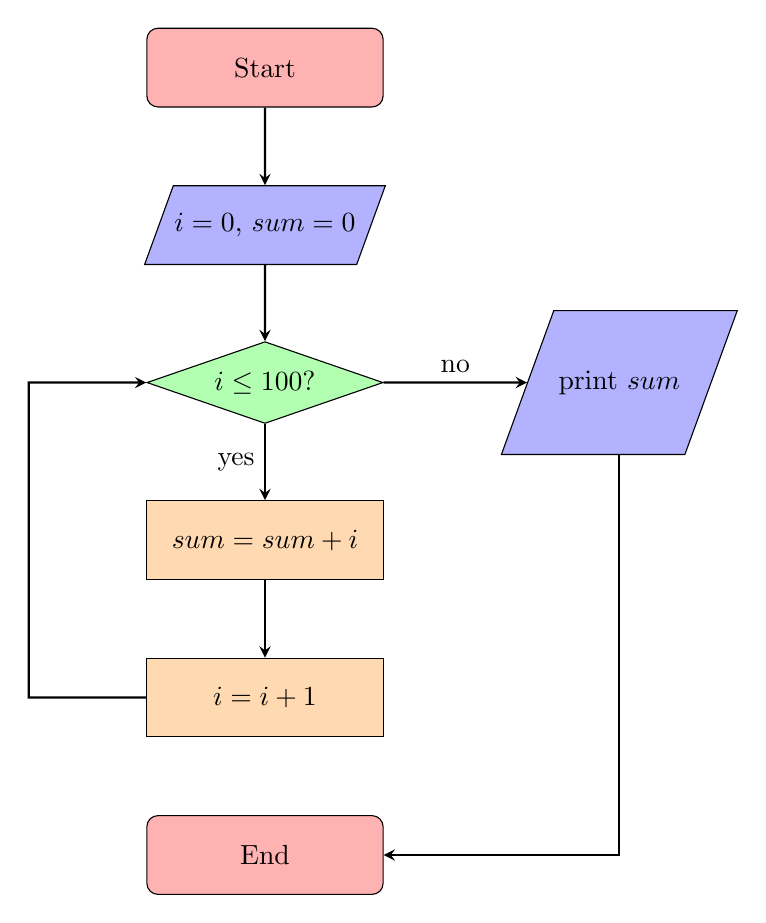
\begin{tikzpicture}[node distance=2cm]
		\node (start) [startend] {Start};
		\node (init) [io, below of=start] {$ i = 0 $, $ sum = 0 $};
		\node (decision)  [decision, below of=init] {$ i \le 100 $?};
		\node (accumulation) [process, below of=decision] {$ sum = sum + i $};
		\node (update) [process, below of=accumulation] {$ i = i + 1 $};
		\node (output) [io, right of=decision, xshift=2.5cm] {print $ sum $};
		\node (end) [startend, below of=update] {End};

		\draw [arrow] (start) -- (init);
		\draw [arrow] (init) -- (decision);
		\draw [arrow] (decision) -- node[anchor=east] {yes } (accumulation);
		\draw [arrow] (accumulation) -- (update);
		\draw [arrow] (update) -- (-3,-8) -- (-3,-4) -- (decision);
		\draw [arrow] (decision) -- node[anchor=south] {no} (output);
		\draw [arrow] (output) |- (end);
	\end{tikzpicture}
	\caption{计算$ \sum_{i=1}^{100} i $的流程图}
\end{figure}

\vspace{0.5cm}

\subsection{Hello World!}

Hello World是学习编程的第一个程序,它的作用是向屏幕输出"Hello World!"。\\

\mybox{Hello World!}

\begin{lstlisting}[language=Python]
print("Hello World!")
\end{lstlisting}

\begin{tcolorbox}
	\mybox{运行结果}
	\begin{verbatim}
Hello World!
	\end{verbatim}
\end{tcolorbox}

不同编程语言的Hello World写法大同小异,可以看出编程语言的基本结构是相似的。\\

\mybox{C}

\begin{lstlisting}[language=C]
#include <stdio.h>

int main() {
	printf("Hello World!\n");
	return 0;
}
\end{lstlisting}

\vspace{0.5cm}

\mybox{C++}

\begin{lstlisting}[language=C++]
#include <iostream>

using namespace std;

int main() {
	cout << "Hello World!" << endl;
	return 0;
}
\end{lstlisting}

\vspace{0.5cm}

\mybox{Java}

\begin{lstlisting}[language=Java]
public class HelloWorld {
    public static void main(String[] args) {
        System.out.println("Hello World!");
    }
}
\end{lstlisting}

\vspace{0.5cm}

\subsection{注释(Comment)}

注释就是对代码的解释和说明,它并不会程序所执行。注释能提高程序的可读性,让人更加容易了解代码的功能。\\

注释一般分为单行注释和多行注释:

\begin{enumerate}
	\item 单行注释:以\#开头,该行之后的内容视为注释。
	\item 多行注释:以"""开头,"""结束,中间的内容视为注释。
\end{enumerate}

\vspace{0.5cm}

\mybox{注释}

\begin{lstlisting}[language=Python]
"""
    Author: Terry
    Date: 2022/11/16
"""
print("Hello World!")       # display "Hello World!"
\end{lstlisting}

\newpage

\section{数据类型}

\subsection{数据类型(Data Types)}

在计算机中,每个数据一般都有一个对应的类型,基础数据类型包括:

\begin{enumerate}
	\item 数值型
	      \begin{itemize}
		      \item 整数int
		      \item 浮点数float
		      \item 复数complex
	      \end{itemize}

	\item 文本型
	      \begin{itemize}
		      \item 字符串str
	      \end{itemize}

	\item 布尔型bool

	\item 数据结构
	      \begin{itemize}
		      \item 列表list
		      \item 元组tuple
		      \item 集合set
		      \item 字典dict
	      \end{itemize}
\end{enumerate}

\vspace{0.5cm}

\subsection{变量(Variable)}

变量是用来存储数据的内存空间,每个变量都有一个类型,使用type()函数可以查看变量的类型。

\vspace{-0.5cm}

\begin{lstlisting}[language=Python]
num = 10;
print(type(num))	# <class 'int'>
salary = 8232.56;
print(type(salary))	# <class 'float'>
\end{lstlisting}

\vspace{0.5cm}

变量的命名需要符合规范:

\begin{enumerate}
	\item 由字母、数字和下划线组成,不能以数字开头
	\item 不可以使用编程语言中预留的关键字
	\item 使用英语单词,顾名思义
\end{enumerate}

关键字是编程语言内置的一些名称,具有特殊的用处和意义,因此不应该作为变量名,防止产生歧义。\\

\begin{table}[H]
	\centering
	\setlength{\tabcolsep}{5mm}{
		\begin{tabular}{|c|c|c|c|c|}
			\hline
			False  & None  & True   & and      & as      \\
			\hline
			assert & break & class  & continue & def     \\
			\hline
			del    & elif  & else   & except   & finally \\
			\hline
			for    & from  & global & if       & import  \\
			\hline
			in     & is    & lambda & nonlocal & not     \\
			\hline
			or     & pass  & raise  & return   & try     \\
			\hline
			while  & with  & yield  &          &         \\
			\hline
		\end{tabular}
	}
	\caption{关键字}
\end{table}

\newpage

\section{输入输出函数}

\subsection{print()}

print()的功能是向屏幕输出指定格式的文本,但是有些需要输出的字符在编程语言中具有特殊含义,因此这些特殊的字符,需要经过转义后输出。\\

\begin{table}[H]
	\centering
	\setlength{\tabcolsep}{5mm}{
		\begin{tabular}{|c|c|}
			\hline
			\textbf{转义字符}      & \textbf{描述}                \\
			\hline
			\lstinline|\\| & 反斜杠\lstinline|\| \\
			\hline
			\lstinline|\'| & 单引号\lstinline|'| \\
			\hline
			\lstinline|\"| & 双引号\lstinline|"| \\
			\hline
			\lstinline|\n| & 换行                         \\
			\hline
			\lstinline|\t| & 制表符                       \\
			\hline
		\end{tabular}
	}
	\caption{转义字符}
\end{table}

\mybox{转义字符}

\begin{lstlisting}[language=Python]
print("\"Hello\nWorld\"")
\end{lstlisting}

\begin{tcolorbox}
	\mybox{运行结果}
	\begin{verbatim}
"Hello
World"
	\end{verbatim}
\end{tcolorbox}

除了直接使用print()输出一个变量的值外,还可以在print()中使用对应类型的占位符。\\

\begin{table}[H]
	\centering
	\setlength{\tabcolsep}{5mm}{
		\begin{tabular}{|c|c|}
			\hline
			\textbf{数据类型} & \textbf{占位符} \\
			\hline
			int               & \%d             \\
			\hline
			float             & \%f             \\
			\hline
			str               & \%s             \\
			\hline
		\end{tabular}
	}
	\caption{占位符}
\end{table}

\vspace{0.5cm}

\mybox{长方形面积}

\begin{lstlisting}[language=Python]
length = 10
width = 5
area = length * width
print("Area = %d * %d = %.2f" % (length, width, area))
\end{lstlisting}

\begin{tcolorbox}
	\mybox{运行结果}
	\begin{verbatim}
Area = 10 * 5 = 50.00
	\end{verbatim}
\end{tcolorbox}

另一种输出的方式是使用f-string,它可以在字符串中直接使用变量的值。

\vspace{-0.5cm}

\begin{lstlisting}[language=Python]
print(f"Area = {length} * {width} = {area:.2f}")
\end{lstlisting}

在默认情况下,print()函数输出数据后,会以换行作为结束符。如果不希望使用换行作为结束符,则可以在print()函数中追加一个end参数。\\

\mybox{等比数列}

\begin{lstlisting}[language=Python]
num1 = 1
num2 = 2
num3 = 4
num4 = 8
print(num1, end=', ')
print(num2, end=', ')
print(num3, end=', ')
print(num4, end='...')
\end{lstlisting}

\begin{tcolorbox}
	\mybox{运行结果}
	\begin{verbatim}
1, 2, 4, 8...
\end{verbatim}
\end{tcolorbox}

\vspace{0.5cm}

\subsection{input()}

有时候一些数据需要从键盘输入,input()可以读取用户输入,并赋值给相应的变量。\\

input()读取到的数据类型是str,通过转换函数可以将其转换为其它类型。\\

\mybox{圆面积}

\begin{lstlisting}[language=Python]
import math

r = float(input("Radius: "))
area = math.pi * r ** 2
print("Area = %.2f" % area)
\end{lstlisting}

\begin{tcolorbox}
	\mybox{运行结果}
	\begin{verbatim}
Radius: 5
Area = 78.54
	\end{verbatim}
\end{tcolorbox}

math模块中定义了一些常用的数学函数,例如pow(x, y)可用于计算$ x $的$ y $次方。\\

\newpage

\section{表达式}

\subsection{算术运算符}

整除运算符//用于计算两个数相除的整数部分,例如21 // 4 = 5。\\

取模(modulo)运算符\%用于计算两个整数相除之后的余数,例如22 \% 3 = 1、4 \% 7 = 4。\\

\mybox{逆序三位数}

\begin{lstlisting}[language=Python]
num = int(input("Enter a 3-digit integer: "))
a = num // 100
b = num // 10 % 10
c = num % 10
print("Reversed:", c * 100 + b * 10 + a)
\end{lstlisting}

\begin{tcolorbox}
	\mybox{运行结果}
	\begin{verbatim}
Enter a 3-digit integer: 520
Reversed: 25
	\end{verbatim}
\end{tcolorbox}

\vspace{0.5cm}

\subsection{复合运算符}

使用复合运算符可以使表达式更加简洁。例如\lstinline|a = a + b|可以写成\lstinline|a += b|,-=、*=、/=、\%=等复合运算符的使用方式同理。\\

\mybox{字符串拼接}

\begin{lstlisting}[language=Python]
s = "Hello" + "World"
s += "!"
print(s)
\end{lstlisting}

\begin{tcolorbox}
	\mybox{运行结果}
	\begin{verbatim}
HelloWorld!
\end{verbatim}
\end{tcolorbox}

\newpage
\chapter{判断}

\section{逻辑运算符}

\subsection{逻辑运算符}

Python中逻辑运算符有三种:

\begin{enumerate}
	\item 逻辑与and:当多个条件同时为真,结果为真。
	      \begin{table}[H]
		      \centering
		      \setlength{\tabcolsep}{5mm}{
			      \begin{tabular}{|c|c|c|}
				      \hline
				      \textbf{条件1} & \textbf{条件2} & \textbf{条件1 and 条件2} \\
				      \hline
				      T              & T              & T                        \\
				      \hline
				      T              & F              & F                        \\
				      \hline
				      F              & T              & F                        \\
				      \hline
				      F              & F              & F                        \\
				      \hline
			      \end{tabular}
		      }
		      \caption{逻辑与}
	      \end{table}

	\item 逻辑或or:多个条件有一个为真时,结果为真。
	      \begin{table}[H]
		      \centering
		      \setlength{\tabcolsep}{5mm}{
			      \begin{tabular}{|c|c|c|}
				      \hline
				      \textbf{条件1} & \textbf{条件2} & \textbf{条件1 or 条件2} \\
				      \hline
				      T              & T              & T                       \\
				      \hline
				      T              & F              & T                       \\
				      \hline
				      F              & T              & T                       \\
				      \hline
				      F              & F              & F                       \\
				      \hline
			      \end{tabular}
		      }
		      \caption{逻辑或}
	      \end{table}

	\item 逻辑非not:条件为真时,结果为假;条件为假时,结果为真。
	      \begin{table}[H]
		      \centering
		      \setlength{\tabcolsep}{5mm}{
			      \begin{tabular}{|c|c|}
				      \hline
				      \textbf{条件} & \textbf{not 条件} \\
				      \hline
				      T             & F                 \\
				      \hline
				      F             & T                 \\
				      \hline
			      \end{tabular}
		      }
		      \caption{逻辑非}
	      \end{table}
\end{enumerate}

\newpage

\section{if}

\subsection{if}

分支结构最大特征就是可以进行指定条件的判断处理,关键字为if、elif、else。\\

每一个满足条件之后的语句都可以有多条,并且在Python里面是利用缩进来确定语句的关系。使用逻辑运算符可以进行若干个条件的连接。

\subsubsection{单分支}

\vspace{-1cm}

\begin{lstlisting}[language=Python]
age = 15
if 0 < age < 18:
    print("未成年")
\end{lstlisting}

\subsubsection{双分支}

\vspace{-1cm}

\begin{lstlisting}[language=Python]
age = 30
if 0 < age < 18:
    print("未成年人")
else:
    print("成年人")
\end{lstlisting}

\subsubsection{多分支}

\vspace{-1cm}

\begin{lstlisting}[language=Python]
score = 76

if 90 <= score <= 100:
    print("优秀")
elif score >= 60:
    print("合格")
else:
    print("不合格")
\end{lstlisting}

\vspace{0.5cm}

\mybox{判断整数奇偶}

\begin{lstlisting}[language=Python]
num = int(input("输入一个正整数:"))

if num > 0:
    if num % 2 == 0:
        print("%d是偶数" % num)
    else:
        print("%d是奇数" % num)
\end{lstlisting}

\begin{tcolorbox}
	\mybox{运行结果}
	\begin{verbatim}
输入一个正整数:66
66是偶数
\end{verbatim}
\end{tcolorbox}

\newpage

\section{断言}

\subsection{断言(Assertion)}

设置断言表达式后,当满足条件时程序正常执行,当断言失败时,程序会中断执行。在进行断言时可以配置错误的提示信息,否则很难知道那块代码出现了错误。\\

通过断言可以直接查找出程序的错误,但从另外一个角度来讲,断言由于不受到程序逻辑的控制,可能会造成许多的额外的问题,在实际的开发之中慎用。\\

\mybox{断言}

\begin{lstlisting}[language=Python]
import math

print("计算三角形面积")
a = float(input("第一条边:"))
b = float(input("第二条边:"))
c = float(input("第三条边:"))

assert a + b > c, "边长不合法"
assert a + c > b, "边长不合法"
assert b + c > a, "边长不合法"

p = (a + b + c) / 2     # 半周长
area = math.sqrt(p * (p-a) * (p-b) * (p-c)) # 海伦公式
print("面积 = %.2f" % area)
\end{lstlisting}

\begin{tcolorbox}
	\mybox{运行结果}
	\begin{verbatim}
计算三角形面积
第一条边:1
第二条边:1
第三条边:2
AssertionError: 边长不合法
\end{verbatim}
\end{tcolorbox}

\newpage
\chapter{循环}

\section{while}

\subsection{while}

while循环会对条件进行判断,如果条件成立,就会执行循环体,然后再次判断条件,直到条件不成立。\\

while循环的次数由循环变量的变化决定,因此while循环一般都包括对循环变量的初值、判断和更新。

\vspace{-0.5cm}

\begin{lstlisting}[language=Python]
i = 1			# initial value
while i <= 5:	# condition
	print("In loop: i =", i)
	i += 1		# update
print("After loop: i =", i)
\end{lstlisting}

while循环的特点是先判断、再执行,因此循环体有可能会执行一次或多次,也有可能一次也不会执行。\\

\mybox{平均身高}

\begin{lstlisting}[language=Python]
NUM_PEOPLE = 5

total = 0

i = 1
while i <= NUM_PEOPLE:
	height = float(input("Enter person %d's height: " % i))
	total += height
	i += 1

average = total / NUM_PEOPLE
print("Average height: %.2f" % average)
\end{lstlisting}

\begin{tcolorbox}
	\mybox{运行结果}
	\begin{verbatim}
Enter person 1's height: 160.8
Enter person 2's height: 175.2
Enter person 3's height: 171.2
Enter person 4's height: 181.3
Enter person 5's height: 164
Average height: 170.50
\end{verbatim}
\end{tcolorbox}

\vspace{0.5cm}

\mybox{整数位数}

\begin{lstlisting}[language=Python]
num = int(input("Enter an integer: "))
n = 0

while num != 0:
	num //= 10
	n += 1

print("Digits:", n)
\end{lstlisting}

\begin{tcolorbox}
	\mybox{运行结果}
	\begin{verbatim}
Enter an integer: 123
Digits: 3
\end{verbatim}
\end{tcolorbox}

\vspace{0.5cm}

\mybox{猜数字}

\begin{lstlisting}[language=Python]
import random

answer = random.randint(1, 100)
cnt = 0

while True:
	num = int(input("Guess a number: "))
	cnt += 1

	if num > answer:
		print("Too high")
	elif num < answer:
		print("Too low")
	else:
		break

print("Correct! You guessed %d times." % cnt)
\end{lstlisting}

\begin{tcolorbox}
	\mybox{运行结果}
	\begin{verbatim}
Guess a number: 50
Too high
Guess a number: 25
Too low
Guess a number: 37
Too low
Guess a number: 43
Too high
Guess a number: 40
Too high
Guess a number: 38
Too low
Guess a number: 39
Correct! You guessed 7 times.
\end{verbatim}
\end{tcolorbox}

\newpage

\section{for}

\subsection{for}

while循环将循环变量的初值、条件和更新写在了三个地方,但是这样不容易明显地看出循环变量的变化。\\

for循环在一行内就可以清晰地表示出循环的次数,因此对于指定次数的循环一般更多地会采用for循环,而对于不确定次数的一般会采用while循环。\\

range()函数能够生成指定范围的整数序列:

\vspace{-0.5cm}

\begin{lstlisting}[language=Python]
for i in range(5):
    print(i, end=' ')		# 0 1 2 3 4

for i in range(10, 15):
	print(i, end=' ')		# 10 11 12 13 14

for i in range(1, 10, 2):
	print(i, end=' ')		# 1 3 5 7 9
\end{lstlisting}

\vspace{0.5cm}

\mybox{累加}

\begin{lstlisting}[language=Python]
sum = 0
for i in range(1, 101):
	sum += i
print("Sum =", sum)
\end{lstlisting}

\begin{tcolorbox}
	\mybox{运行结果}
	\begin{verbatim}
Sum = 5050
\end{verbatim}
\end{tcolorbox}

\vspace{0.5cm}

\mybox{斐波那契数列}

\begin{figure}[H]
	\centering
	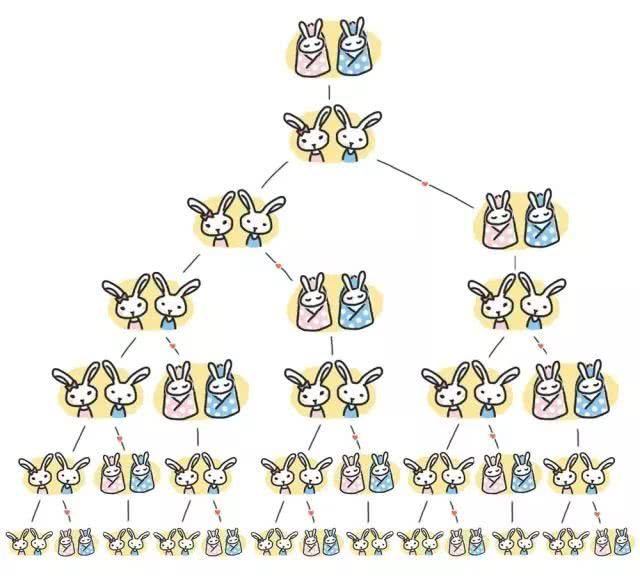
\includegraphics[scale=0.5]{img/Chapter3/3-2/1.png}
\end{figure}

\begin{lstlisting}[language=Python]
n = int(input("Enter the number of terms: "))

if n == 1:
	print(1)
elif n == 2:
	print(1, 1)
else:
	num1 = 1
	num2 = 1
	print(1, 1, end=' ')
	for i in range(3, n + 1):
		val = num1 + num2
		print(val, end=' ')
		num1 = num2
		num2 = val
	print()
\end{lstlisting}

\begin{tcolorbox}
	\mybox{运行结果}
	\begin{verbatim}
Enter the number of terms: 10
1 1 2 3 5 8 13 21 34 55
\end{verbatim}
\end{tcolorbox}

\vspace{0.5cm}

\subsection{嵌套循环}

循环也可以嵌套使用,外层循环每执行一次,内层循环就会执行多次。

\vspace{-0.5cm}

\begin{lstlisting}[language=Python]
for i in range(2):
	for j in range(3):
		print("i = %d, j = %d" % (i, j))
\end{lstlisting}

\begin{tcolorbox}
	\mybox{运行结果}
	\begin{verbatim}
i = 0, j = 0
i = 0, j = 1
i = 0, j = 2
i = 1, j = 0
i = 1, j = 1
i = 1, j = 2
\end{verbatim}
\end{tcolorbox}

\vspace{0.5cm}

\mybox{九九乘法表}\\

\begin{table}[H]
	\centering
	\setlength{\tabcolsep}{1.5mm}{
		\begin{tabular}{|c|c|c|c|c|c|c|c|c|}
			\hline
			1*1=1 & 1*2=2  & 1*3=3  & 1*4=4  & 1*5=5  & 1*6=6  & 1*7=7  & 1*8=8  & 1*9=9  \\
			\hline
			2*1=2 & 2*2=4  & 2*3=6  & 2*4=8  & 2*5=10 & 2*6=12 & 2*7=14 & 2*8=16 & 2*9=18 \\
			\hline
			3*1=3 & 3*2=6  & 3*3=9  & 3*4=12 & 3*5=15 & 3*6=18 & 3*7=21 & 3*8=24 & 3*9=27 \\
			\hline
			4*1=4 & 4*2=8  & 4*3=12 & 4*4=16 & 4*5=20 & 4*6=24 & 4*7=28 & 4*8=32 & 4*9=36 \\
			\hline
			5*1=5 & 5*2=10 & 5*3=15 & 5*4=20 & 5*5=25 & 5*6=30 & 5*7=35 & 5*8=40 & 5*9=45 \\
			\hline
			6*1=6 & 6*2=12 & 6*3=18 & 6*4=24 & 6*5=30 & 6*6=36 & 6*7=42 & 6*8=48 & 6*9=54 \\
			\hline
			7*1=7 & 7*2=14 & 7*3=21 & 7*4=28 & 7*5=35 & 7*6=42 & 7*7=49 & 7*8=56 & 7*9=63 \\
			\hline
			8*1=8 & 8*2=16 & 8*3=24 & 8*4=32 & 8*5=40 & 8*6=48 & 8*7=56 & 8*8=64 & 8*9=72 \\
			\hline
			9*1=9 & 9*2=18 & 9*3=27 & 9*4=36 & 9*5=45 & 9*6=54 & 9*7=63 & 9*8=72 & 9*9=81 \\
			\hline
		\end{tabular}
	}
\end{table}

\begin{lstlisting}[language=Python]
for i in range(1, 10):
    for j in range(1, 10):
        print("%d*%d=%d\t" % (i, j, i * j), end='')
    print()
\end{lstlisting}

\vspace{0.5cm}

\mybox{打印图案}

\begin{lstlisting}
*
**
***
****
*****
\end{lstlisting}

\begin{lstlisting}[language=Python]
for i in range(1, 6):
	for j in range(1, i + 1):
		print("*", end='')
	print()
\end{lstlisting}

\newpage

\section{break or continue?}

\subsection{break}

break可用于跳出当前的switch或循环结构。在一些情况下,在循环的中途已经完成了某个目标,没有必要再进行剩余的循环,这时就可以使用break跳出循环。\\

例如在判断一个数$ n $是否为素数时,利用循环逐个判断$ 2 \sim n - 1 $之间的数是否能整除$ n $。只要发现其中有一个数能整除$ n $,就证明$ n $不是素数,可以跳出循环,不必再进行剩余的检查。\\

\mybox{素数}

\begin{lstlisting}[language=Python]
import math

n = int(input("Enter an integer: "))

is_prime = True
for i in range(2, int(math.sqrt(n)) + 1):
	if n % i == 0:
		is_prime = False
		break

if is_prime:
	print(n, "is a prime number")
else:
	print(n, "is not a prime number")
\end{lstlisting}

\begin{tcolorbox}
	\mybox{运行结果}
	\begin{verbatim}
Enter an integer: 17
17 is a prime number
\end{verbatim}
\end{tcolorbox}

\vspace{0.5cm}

\subsection{continue}

continue与break使用方法类似,但是它并不是跳出循环,而是跳过本轮循环,直接开始下一轮循环。\\

\mybox{正数平方和}

\begin{lstlisting}[language=Python]
n = 10
print("Enter %d integers: " % n)

sum_square = 0
for i in range(n):
	num = int(input())
	if num < 0:
		continue
	sum_square += num * num

print("Sum of squares of positive integers:", sum_square)
\end{lstlisting}

\begin{tcolorbox}
	\mybox{运行结果}
	\begin{verbatim}
Enter 10 integers: 
5 
7
-2
0
4
-4
-9
3
9
5
Sum of squares of positive integers: 205
\end{verbatim}
\end{tcolorbox}

\newpage
\chapter{数据结构}

\section{序列}

\subsection{序列}

Python中序列类型包含字符串、列表、元组、字典。序列的核心意义在于可以进行多个数据的保存。\\

Python在整体设计的过程之中强调的是简单化。以多数据的存储为例,在许多的编程语言里面,都是利用了数组实现了数据的存储,但是数据有一个最大的问题在于:长度是固定的,无法进行容量的扩充。\\

在这样的背景下,很多的开发者就不得不去独立地进行一些动态数组的开发,所以就有了数据结构的概念,而数据存储的内容多了,就需要提升数据的操作性能,C、C++、Java等等都有这样的问题。\\

Python在设计的时候充分地考虑到了这些动态性的设计问题,所以才将这些可能动态修改的内容统一地称为序列,也就是说Python中的序列就是一个动态(或静态)的存储,而这些存储的操作结构都是内置的,开发者可以避免数据结构的开发所造成的困难,尤其是面对与非科班的人而言。\\

列表是对传统数组的一种使用包装,但是与传统数组最大的不同在于,Python中的列表的内容是允许进行动态修改的,并且Python中的列表也可以像传统数组那样机型索引的访问,这样就使得时间复杂度降低了许多。

\newpage

\section{列表}

\subsection{列表(List)}

列表使用【[]】进行列表的定义,Python的列表是对于传统数组的更高级的实现。列表可以通过索引的形式进行访问,索引下标是从0开始的,到列表长度 - 1结束。\\

在使用列表进行数据存储的时候,虽然大部分的情况下都会使用相同的数据类型,但是在列表里面却可以同时有不同的数据类型,这比其它语言里面提供的数据的功能强大。虽然提供有多个数据类型的保存使得程序存储更加灵活,但是从实际的开发角度而言,尽量让数据类型保持一致会比较合理。\\

在Python中列表除了正向索引访问之外,也可以进行反向索引访问。\\

\mybox{列表}

\begin{lstlisting}[language=Python]
lst = [1, 2, 3]

print(lst[0])
print(lst[1])
print(lst[2])

print(lst[-1])
print(lst[-2])
print(lst[-3])

print(lst[3])       # 越界
\end{lstlisting}

\begin{tcolorbox}
	\mybox{运行结果}
	\begin{verbatim}
1
2
3
3
2
1
IndexError: list index out of range
\end{verbatim}
\end{tcolorbox}

序列数据可以直接使用【*】进行重复定义,或者使用【+】进行与其它序列拼接。\\

\mybox{序列重复/拼接}

\begin{lstlisting}[language=Python]
lst = [1, 2, 3] * 3
print(lst)      # [1, 2, 3, 1, 2, 3, 1, 2, 3]

lst = [1, 2, 3] + [4, 5, 6]
print(lst)      # [1, 2, 3, 4, 5, 6]
\end{lstlisting}

\begin{tcolorbox}
	\mybox{运行结果}
	\begin{verbatim}
[1, 2, 3, 1, 2, 3, 1, 2, 3]
[1, 2, 3, 4, 5, 6]
\end{verbatim}
\end{tcolorbox}

\vspace{0.5cm}

\subsection{成员运算符}

在使用索引访问的时候都需要去考虑索引的设置错误的问题,但是使用了for循环之后,不再需要明确的进行索引的设置,避免了IndexError异常信息。\\

如果想要判断某一个数据是否在列表之中存在,最直接的方式就是直接进行列表的迭代操作(其它语言传统形式)。\\

\mybox{迭代查找}

\begin{lstlisting}[language=Python]
lst = ["C/C++", "Java", "Python", "JavaScript"]
key = "Python"      # 待查找关键词
flag = False        # 初始假设未找到

for item in lst:
    if item == key:
        flag = True
        break

if flag:
    print("数据存在")
else:
    print("数据不存在")
\end{lstlisting}

\begin{tcolorbox}
	\mybox{运行结果}
	\begin{verbatim}
数据存在
\end{verbatim}
\end{tcolorbox}

这种查询最大的问题在于需要进行整个列表数据的迭代,造成的结果就是时间复杂度的攀升$ O(n) $。在Python设计过程之中不希望开发者为这些复杂的执行效率犯愁,所以在使用列表判断某些数据是否存在的时候提供了专门的运算符。使用关键字in(在范围内)、not in(不在范围内)。\\

\mybox{成员运算符}

\begin{lstlisting}[language=Python]
lst = ["C/C++", "Java", "Python", "JavaScript"]
key = "Python"      # 待查找关键词

if key in lst:
    print("数据存在")
else:
    print("数据不存在")
\end{lstlisting}

\begin{tcolorbox}
	\mybox{运行结果}
	\begin{verbatim}
数据存在
\end{verbatim}
\end{tcolorbox}

\vspace{0.5cm}

\subsection{切片(Splicing)}

切片可以截取部分的列表内容。在默认情况下,数据的分片都是依照数值为1的间隔进行获取的,如果有需要也可以进行步长的修改。\\

\mybox{切片}

\begin{lstlisting}[language=Python]
lst = list(range(10))

print("原始列表:", end='')
print(lst)

print("截取[2:7]:", end='')
print(lst[2:7])

print("截取[:5]:", end='')
print(lst[:5])

print("截取[3:]:", end='')
print(lst[3:])

print("截取[::2]:", end='')
print(lst[::2])
\end{lstlisting}

\begin{tcolorbox}
	\mybox{运行结果}
	\begin{verbatim}
原始列表:[0, 1, 2, 3, 4, 5, 6, 7, 8, 9]
截取[2:7]:[2, 3, 4, 5, 6]
截取[:5]:[0, 1, 2, 3, 4]
截取[3:]:[3, 4, 5, 6, 7, 8, 9]
截取[::2]:[0, 2, 4, 6, 8]
\end{verbatim}
\end{tcolorbox}

\vspace{0.5cm}

\subsection{列表操作函数}

Python中的列表设计非常到位,它可以实现内容动态扩充,可以进行后期的追加或者删除。

\begin{table}[H]
	\centering
	\setlength{\tabcolsep}{5mm}{
		\begin{tabular}{|l|l|}
			\hline
			\textbf{函数}       & \textbf{功能}                    \\
			\hline
			append(data)        & 在列表最后追加新内容             \\
			\hline
			clear()             & 清除列表数据                     \\
			\hline
			copy()              & 列表拷贝                         \\
			\hline
			count()             & 统计某一个数据在列表中的出现次数 \\
			\hline
			extend(列表)        & 为一个列表追加另外一个列表       \\
			\hline
			index(data)         & 从列表查询某个值第一次出现的位置 \\
			\hline
			insert(index, data) & 向列表中指定索引位置追加新数据   \\
			\hline
			pop(index)          & 从列表弹出并删除一个数据         \\
			\hline
			remove(data)        & 从列表删除数据                   \\
			\hline
			reverse()           & 列表数据反转                     \\
			\hline
			sort()              & 列表数据排序                     \\
			\hline
		\end{tabular}
	}
	\caption{列表操作函数}
\end{table}

\vspace{0.5cm}

\mybox{列表内容扩充}

\begin{lstlisting}[language=Python]
lst = list(range(5))    # [0, 1, 2, 3, 4]
lst.append(5)           # [0, 1, 2, 3, 4, 5]
lst.insert(2, 6)        # [0, 1, 6, 2, 3, 4, 5]
print(lst)
print("列表长度:%d" % len(lst))
\end{lstlisting}

\begin{tcolorbox}
	\mybox{运行结果}
	\begin{verbatim}
[0, 1, 6, 2, 3, 4, 5]
列表长度:7
\end{verbatim}
\end{tcolorbox}

在使用remove()删除的时候,内容存在可以删除,不存在就会抛出ValueError异常信息,因此使用remove()操作之前一定要通过in判断。\\

如果不知道内容要进行数据的删除,最简单的原始的Python支持可以采用del关键字实现内容删除,而且使用del的时候只需要知道列表数据的索引即可实现。使用del关键字的确可以实现索引的删除,但是无法知道被删除了哪些数据。\\

pop()可以根据索引删除,而后告诉用户哪些数据被删除了。\\

\mybox{删除元素}

\begin{lstlisting}[language=Python]
lst = list(range(5))    # [0, 1, 2, 3, 4]
key = 3

if key in lst:
    lst.remove(key)
print(lst)              # [0, 1, 2, 4]

del lst[2]
print(lst)              # [0, 1, 4]

print(lst.pop(1))       # 1
print(lst)              # [0, 4]
\end{lstlisting}

\begin{tcolorbox}
	\mybox{运行结果}
	\begin{verbatim}
[0, 1, 2, 4]
[0, 1, 4]
1
[0, 4]
\end{verbatim}
\end{tcolorbox}

\vspace{0.5cm}

\mybox{列表反转/排序}

\begin{lstlisting}[language=Python]
lst = [7, 4, 0, 3, 6, 8, 9, 2]

print("原始列表:", end='')
print(lst)

print("反转:", end='')
lst.reverse()
print(lst)

print("排序(升序):", end='')
lst.sort()
print(lst)

print("排序(降序):", end='')
lst.sort(reverse=True)
print(lst)
\end{lstlisting}

\begin{tcolorbox}
	\mybox{运行结果}
	\begin{verbatim}
原始列表:[7, 4, 0, 3, 6, 8, 9, 2]
反转:[2, 9, 8, 6, 3, 0, 4, 7]
排序(升序):[0, 2, 3, 4, 6, 7, 8, 9]
排序(降序):[9, 8, 7, 6, 4, 3, 2, 0]
\end{verbatim}
\end{tcolorbox}

\newpage

\section{元组}

\subsection{元组(Tuple)}

列表是可以进行多个数据的保存,并且里面的内容都是可以修改和动态扩充的。与列表不一样,Python提供了一个不可变的数据的序列——元组,元组需要使用【()】进行定义。元组定义的时候如果只有一个内容,必须要有【,】。\\

\mybox{元组}

\begin{lstlisting}[language=Python]
tup = (0, 1, 2, 3, 4)
print(tup)
tup[0] = 5
\end{lstlisting}

\begin{tcolorbox}
	\mybox{运行结果}
	\begin{verbatim}
(0, 1, 2, 3, 4)
TypeError: 'tuple' object does not support item assignment
\end{verbatim}
\end{tcolorbox}

tuple()可以实现列表与元组的转换。\\

\mybox{元组与列表的转换}

\begin{lstlisting}[language=Python]
lst = list(range(5))
print(lst)
print(type(lst))

tup = tuple(lst)
print(tup)
print(type(tup))
\end{lstlisting}

\begin{tcolorbox}
	\mybox{运行结果}
	\begin{verbatim}
[0, 1, 2, 3, 4]
<class 'list'>
(0, 1, 2, 3, 4)
<class 'tuple'>
\end{verbatim}
\end{tcolorbox}

\vspace{0.5cm}

\subsection{序列统计函数}

\begin{table}[H]
	\centering
	\setlength{\tabcolsep}{5mm}{
		\begin{tabular}{|l|l|}
			\hline
			\textbf{函数} & \textbf{功能}                              \\
			\hline
			len()         & 获取序列的长度                             \\
			\hline
			max()         & 获取序列中的最大值                         \\
			\hline
			min()         & 获取序列中的最小值                         \\
			\hline
			sum()         & 计算序列中的内容总和                       \\
			\hline
			any()         & 序列中有一个为True结果为True,否则为False  \\
			\hline
			all()         & 序列中有一个为False结果为False,否则为True \\
			\hline
		\end{tabular}
	}
	\caption{序列统计函数}
\end{table}

\vspace{0.5cm}

\mybox{序列统计函数}

\begin{lstlisting}[language=Python]
lst = [4, 0, 1, 3, 2]
tup = (8, 5, 7, 9, 6)
str = "HelloWorld"

print("列表lst的长度 = %d" % len(lst))
print("元组tup的长度 = %d" % len(tup))
print("字符串str的长度 = %d" % len(str))

print("列表lst最大值:%d" % max(lst))
print("元组tup最小值 = %d" % min(tup))
print("字符串str最大值 = %c" % max(str))
print("字符串str最小值 = %c" % min(str))

print("列表lst总和:%d" % sum(lst))
print("元组tup总和:%d" % sum(tup))
\end{lstlisting}

\begin{tcolorbox}
	\mybox{运行结果}
	\begin{verbatim}
列表lst的长度 = 5
元组tup的长度 = 5
字符串str的长度 = 10
列表lst最大值:4
元组tup最小值 = 5
字符串str最大值 = r
字符串str最小值 = H
列表lst总和:10
元组tup总和:35
\end{verbatim}
\end{tcolorbox}

\newpage

\section{字符串}

\subsection{字符串(String)}

字符串是由若干个字符所组成的,使用引号进行一串内容的声明。字符串也可以进行数据的分片操作和序列统计函数。\\

\mybox{字符串}

\begin{lstlisting}[language=Python]
info = "url: www.baidu.com"

print("字符串长度:%d" % len(info))

if "url: " in info:
    print(info[5:])
\end{lstlisting}

\begin{tcolorbox}
	\mybox{运行结果}
	\begin{verbatim}
字符串长度:18
www.baidu.com
\end{verbatim}
\end{tcolorbox}

\vspace{0.5cm}

\subsection{字符串格式化}

在Python默认的语言环境中有字符串格式化的处理支持。为了进一步完善对于字符串格式化的需求,又提供了format()。在format()里面出现的【\{\}】标记里面可以定义标记名称或者数据的填充序列顺序定义。\\

\mybox{字符串格式化}

\begin{lstlisting}[language=Python]
name = "小灰"
age = 16
height = 175.6

info = "姓名:%s,年龄:%d,身高:%.2f" % (name, age, height)
print(info)

info = "姓名:{},年龄:{},身高:{}".format(name, age, height)
print(info)
\end{lstlisting}

\begin{tcolorbox}
	\mybox{运行结果}
	\begin{verbatim}
姓名:小灰,年龄:16,身高:175.60
姓名:小灰,年龄:16,身高:175.6
\end{verbatim}
\end{tcolorbox}

\vspace{0.5cm}

\subsection{字符串数据处理函数}

\begin{table}[H]
	\centering
	\setlength{\tabcolsep}{5mm}{
		\begin{tabular}{|l|l|}
			\hline
			\textbf{函数}               & \textbf{功能}                        \\
			\hline
			center()                    & 字符串居中显示                       \\
			\hline
			find(data)                  & 查找到内容返回索引位置,找不到返回-1 \\
			\hline
			join(data)                  & 字符串连接                           \\
			\hline
			split(data [, limit])       & 字符串拆分                           \\
			\hline
			lower()                     & 字符串转小写                         \\
			\hline
			upper()                     & 字符串转大写                         \\
			\hline
			capitalize()                & 首字母大写                           \\
			\hline
			replace(old, new [, limit]) & 字符串替换                           \\
			\hline
			strip()                     & 删除左右空格                         \\
			\hline
		\end{tabular}
	}
	\caption{字符串数据处理函数}
\end{table}

\subsubsection{字符串大小写转换}

\vspace{0.5cm}

\mybox{字符串大小写转换}

\begin{lstlisting}[language=Python]
str = "Hello World!"
print(str.upper())
print(str.lower())
\end{lstlisting}

\begin{tcolorbox}
	\mybox{运行结果}
	\begin{verbatim}
HELLO WORLD!
hello world!
\end{verbatim}
\end{tcolorbox}

\subsubsection{字符串查找find()}

在进行数据内容查询的时候,如果内容存在就返回索引位置,不存在则返回-1。\\

\mybox{字符串查找}

\begin{lstlisting}[language=Python]
str = "Hello World!"
print(str.find("Wor"))
print(str.find("Python"))
\end{lstlisting}

\begin{tcolorbox}
	\mybox{运行结果}
	\begin{verbatim}
6
-1
\end{verbatim}
\end{tcolorbox}

\subsubsection{字符串连接join()}

使用一个特定的字符串连接序列中的若干内容。\\

\mybox{字符串连接}

\begin{lstlisting}[language=Python]
lst = ["www", "baidu", "com"]
url = ".".join(lst)
print(url)
\end{lstlisting}

\begin{tcolorbox}
	\mybox{运行结果}
	\begin{verbatim}
www.baidu.com
\end{verbatim}
\end{tcolorbox}

\subsubsection{字符串拆分split()}

\vspace{0.5cm}

\mybox{字符串拆分}

\begin{lstlisting}[language=Python]
ip = "127.0.0.1"
print("ip信息:%s" % ip.split("."))

date_time = "2021/03/31 17:32:53"
item = date_time.split(" ")
print("date信息:%s" % item[0].split("/"))
print("time信息:%s" % item[1].split(":"))
\end{lstlisting}

\begin{tcolorbox}
	\mybox{运行结果}
	\begin{verbatim}
ip信息:['127', '0', '0', '1']
date信息:['2021', '03', '31']
time信息:['17', '32', '53']
\end{verbatim}
\end{tcolorbox}

\subsubsection{字符串替换replace()}

使用一个字符串去替换其它的字符串,在进行字符串替换的时候可以设置替换的次数。replace()的替换是进行全匹配的替换操作。\\

\mybox{字符串替换}

\begin{lstlisting}[language=Python]
str = "Hello World, Hello Python!"
print("全部替换:" + str.replace("Hello", "Hey"))
print("部分替换:" + str.replace("Hello", "Hey", 1))
\end{lstlisting}

\begin{tcolorbox}
	\mybox{运行结果}
	\begin{verbatim}
全部替换:Hey World, Hey Python!
部分替换:Hey World, Hello Python!
\end{verbatim}
\end{tcolorbox}

\subsubsection{字符串去除前后空格strip()}

在用户键盘数据输入的过程中,有可能用户在输入信息时会添加无用的空格,导致数据判断错误。对于用户输入数据需要进行左右空格的删除。\\

\mybox{模拟登陆}

\begin{lstlisting}[language=Python]
while True:
    info = input("Username:Password >>> ")
    if len(info) == 0 or info.find(":") == -1:
        print("输入格式错误!")
    else:
        data = info.split(":")
        username = data[0]
        password = data[1]
        if username == "admin" and password == "123456":
            print("欢迎【%s】成功登录!" % username)
            break
        else:
            print("用户名或密码错误!")
\end{lstlisting}

\begin{tcolorbox}
	\mybox{运行结果}
	\begin{verbatim}
Username:Password >>> hey:
用户名或密码错误!
Username:Password >>> admin
输入格式错误!
Username:Password >>> admin:123456
欢迎【admin】成功登录!
\end{verbatim}
\end{tcolorbox}

\newpage

\section{字典}

\subsection{字典(Dictionary)}

字典是一个在开发之中极为重要的类型,字典提供了非常方便地数据内容查找操作。字典的本质就是一个数据查找的序列,与之前的列表或者元组不同的地方在于,其它的结构保存数据的目的都是为了输出使用,而字典是为了查询使用。\\

字典严格意义上来讲属于一种哈希表的结构,在哈希表进行数据存储的时候往往都需要一个哈希算法进行数据存储位置的计算。\\

字典是一个二元偶对象的集合,所以里面保存的数据都是成对的,所有的数据内容都按照key = value的形式进行存放。考虑到用户使用的方便,key的类型可以使数字、字符串或者是元组,但是最为常见的还是字符串。\\

在使用字典进行查询的时候如果指定的key不存在,则在代码执行会出现KeyError错误提示信息,也就是原生的数据查询方式是有可能会抛出异常的。\\

字典的本质是根据key查找对应的value,一旦key重复的时候,使用新的数据覆盖掉旧的数据。\\

\mybox{字典}

\begin{lstlisting}[language=Python]
info = {"name": "小灰", "age": 16, "height": 175.6}
print(info)
print(info["age"])

info["height"] = 180
print(info)
\end{lstlisting}

\begin{tcolorbox}
	\mybox{运行结果}
	\begin{verbatim}
{'name': '小灰', 'age': 16, 'height': 175.6}
16
{'name': '小灰', 'age': 16, 'height': 180}
\end{verbatim}
\end{tcolorbox}

既然字典是一个序列,那么字典可以使用in进行判断指定key是否存在,通过这样的机制可以避免由于key不存在所带来的KeyError异常的抛出。\\


同样,字典也可以使用for循环迭代输出,但是迭代的知识字典中全部的key。\\

\mybox{字典迭代输出}

\begin{lstlisting}[language=Python]
info = {"name": "小灰", "age": 16, "height": 175.6}
for key in info:
    print("%s: %s" % (key, info[key]))
\end{lstlisting}

\begin{tcolorbox}
	\mybox{运行结果}
	\begin{verbatim}
name: 小灰
age: 16
height: 175.6
\end{verbatim}
\end{tcolorbox}

在进行字典数据迭代输出的时候,最好的做法是每一次迭代直接返回当前完整的key:value的映射项,此时的处理就需要依赖items()来完成。\\

\mybox{items()迭代输出}

\begin{lstlisting}[language=Python]
info = {"name": "小灰", "age": 16, "height": 175.6}
for key, value in info.items():
    print("%s: %s" % (key, value))
\end{lstlisting}

\begin{tcolorbox}
	\mybox{运行结果}
	\begin{verbatim}
name: 小灰
age: 16
height: 175.6
\end{verbatim}
\end{tcolorbox}

\vspace{0.5cm}

\subsection{字典操作函数}

\begin{table}[H]
	\centering
	\setlength{\tabcolsep}{5mm}{
		\begin{tabular}{|l|l|}
			\hline
			\textbf{函数}            & \textbf{功能}             \\
			\hline
			clear()                  & 清空字典数据              \\
			\hline
			update(\{k:v, ...\})     & 更新字典数据              \\
			\hline
			get(key[, defaultvalue]) & 根据key获取数据           \\
			\hline
			pop(key)                 & 弹出字典中指定的key数据   \\
			\hline
			popitem()                & 从字典中弹出一组映射项    \\
			\hline
			keys()                   & 返回字典中全部key数据     \\
			\hline
			values()                 & 返回字典中全部的value数据 \\
			\hline
		\end{tabular}
	}
	\caption{字典操作函数}
\end{table}

\subsubsection{字典数据更新update()}

Python中的字典是可以进行存储数据的动态扩充的,update()除了拥有表面上的更新之外,也拥有数据的扩充操作。\\

\mybox{字典数据更新update()}

\begin{lstlisting}[language=Python]
info = {"name": "小灰", "age": 16, "height": 175.6}
info.update({"city": "Shanghai", "job": "programmer"})
print(info)
\end{lstlisting}

\begin{tcolorbox}
	\mybox{运行结果}
	\begin{verbatim}
{'name': '小灰', 'age': 16, 'height': 175.6,
'city': 'Shanghai', 'job': 'programmer'}
\end{verbatim}
\end{tcolorbox}

\subsubsection{字典数据删除pop()}

pop()可以根据key进行弹出操作。\\

\mybox{字典数据删除}

\begin{lstlisting}[language=Python]
info = {"name": "小灰", "age": 16, "height": 175.6}
print(info.pop("age"))
print(info)
\end{lstlisting}

\begin{tcolorbox}
	\mybox{运行结果}
	\begin{verbatim}
16
{'name': '小灰', 'height': 175.6}
\end{verbatim}
\end{tcolorbox}

\subsubsection{字典数据获取get()}

可以通过key获取数据,如果key不存在则返回None。\\

\mybox{字典数据获取}

\begin{lstlisting}[language=Python]
info = {"name": "小灰", "age": 16, "height": 175.6}
print(info.get("name"))
print(info.get("job"))
\end{lstlisting}

\begin{tcolorbox}
	\mybox{运行结果}
	\begin{verbatim}
小灰
None
\end{verbatim}
\end{tcolorbox}

\newpage
\chapter{函数}

\section{函数}

\subsection{函数(Function)}

数学中的函数$ y = f(x) $,通过输入$ x $的值,经过计算可以得到$ y $的值。计算机中的函数也是如此,将输入传给函数,经过处理后,会得到输出。\\

函数是一段可重复使用的代码,做了一个特定的任务。例如print()和len()就是函数,其中print()的功能是输出字符串,len()的功能是序列的长度。\\

\begin{figure}[H]
	\centering
	\begin{tikzpicture}[scale=0.5]
		\draw[-] (5,-2) -- (10,-2) -- (10,2) -- (5,2) -- (5,-2);
		\draw[->] (0,0) -- (5,0);
		\draw[->] (10,0) -- (15,0);

		\draw (-2,0) node {Input};
		\draw (17,0) node {Output};
		\draw (7.5,0) node {Function};
	\end{tikzpicture}
	\caption{函数}
\end{figure}

除了这些内置的函数以外,开发者还可以自定义函数,将程序中会被多次使用的代码或做了一件特定的任务的代码写成一个函数,这样就能避免重复写相同的代码,提高开发效率,也利于维护。\\

在编写函数时需要:

\begin{enumerate}
	\item 确定函数的功能
	      \begin{itemize}
		      \item 函数名
		      \item 确保一个函数只做一件事
	      \end{itemize}

	\item 确定函数的输入(参数)
	      \begin{itemize}
		      \item 是否需要参数
		      \item 参数个数
		      \item 参数类型
	      \end{itemize}

	\item 确定函数的输出(返回值)
	      \begin{itemize}
		      \item 是否需要返回值
		      \item 返回值类型
	      \end{itemize}
\end{enumerate}

\vspace{0.5cm}

\mybox{最大值}

\begin{lstlisting}[language=Python]
def max(num1, num2):
    # if num1 > num2:
    #     return num1
    # else:
    #     return num2

    return num1 if num1 > num2 else num2

print(max(4, 12))
print(max(54, 33))
print(max(-999, -774))
\end{lstlisting}

\begin{tcolorbox}
	\mybox{运行结果}
	\begin{verbatim}
12
54
-774
	\end{verbatim}
\end{tcolorbox}

函数也可以没有返回值,因为它执行完函数后,并不需要将结果返回给调用者。\\

\mybox{棋盘}

\begin{lstlisting}[language=Python]
def print_board():
    for i in range(3):
        for j in range(2):
            print("   |", end='')
        print()
        if i < 2:
            print("---+---+---")

print_board()
\end{lstlisting}

\begin{tcolorbox}
	\mybox{运行结果}
	\begin{verbatim}
   |   |
---+---+---
   |   |
---+---+---
   |   |
	\end{verbatim}
\end{tcolorbox}

\vspace{0.5cm}

\subsection{函数调用}

当调用函数时,程序会记录下当前的执行位置,并跳转到被调用的函数处执行。当被调用的函数执行结束后,程序会回到之前的位置继续执行。\\

\begin{figure}[H]
	\centering
	\begin{tikzpicture}[]
		\draw (0,4.5) node {Caller};
		\draw[->] (0,4) -- (0,0.5);
		\draw[->] (0,-0.5) -- (0,-4);
		\draw (0,0) node {调用foo()};

		\draw (4,4) node {foo()};
		\draw[->] (4,3) -- (4,0.5);
		\draw[->] (4,-0.5) -- (4,-3);
		\draw (4,0) node {调用bar()};

		\draw (8,3) node {bar()};
		\draw[->] (8,2) -- (8,-2);

		\draw[->] (0.5,0.5) -- (3.5,3);
		\draw[->] (3.5,-3) -- (0.5,-0.5);
		\draw[->] (4.5,0.5) -- (7.5,2);
		\draw[->] (7.5,-2) -- (4.5,-0.5);
	\end{tikzpicture}
	\caption{函数调用}
\end{figure}

\vspace{0.5cm}

\mybox{两点间距离}

\begin{lstlisting}[language=Python]
import math

def square(x):
	return x ** 2
	
def distance(point1, point2):
	x1, y1 = point1
	x2, y2 = point2
	return math.sqrt(square(x1 - x2) + square(y1 - y2))
	
x1, y1 = eval(input("Enter (x1, y1): "))
x2, y2 = eval(input("Enter (x2, y2): "))
print("Distance:", distance((x1, y1), (x2, y2)))
\end{lstlisting}

\begin{tcolorbox}
	\mybox{运行结果}
	\begin{verbatim}
Enter (x1, y1): 0, 0
Enter (x2, y2): 3, 4
Distance: 5.0
	\end{verbatim}
\end{tcolorbox}

\vspace{0.5cm}

\subsection{main()}

很多编程语言都使用main()函数作为程序的入口,在Python中main()并不是必须的,但是使用main()函数可以使代码的结构更加清晰。\\

\_\_name\_\_是一个内置变量,当文件作为程序执行时,其值为\_\_main\_\_。

\vspace{-0.5cm}

\begin{lstlisting}[language=Python]
def main():
    pass

if __name__ == "__main__":
    main()
\end{lstlisting}

\newpage

\section{作用域}

\subsection{局部变量(Local Variable)}

定义在块中的变量称为局部变量,它只能在块中访问。当代码块结束时,局部变量就会被销毁。因此,局部变量的生命周期为从声明时开始到所在块结束。\\

块与块之间的局部变量是互相独立的,即使变量名相同,它们也不是同一个变量。\\

例如在函数调用中,函数的参数也是局部变量,它们的作用域仅限于函数内。\\

例如一个用于交换两个变量的函数swap(),在main()中的变量a和b与swap()中的a和b并不是同一个变量。在调用swap()时,是将main()中的a和b的值复制给swap()中的a和b。swap()交换的是其内部的局部变量,并不会对main()中的a和b产生任何影响。\\

\mybox{局部变量}

\begin{lstlisting}[language=Python]
def swap(a, b):
    a, b = b, a
    print("swap(): a = %d, b = %d" % (a, b))

def main():
    a, b = 1, 2

    print("Before: a = %d, b = %d" % (a, b))
    swap(a, b)
    print("After: a = %d, b = %d" % (a, b))

if __name__ == "__main__":
    main()
\end{lstlisting}

\begin{tcolorbox}
	\mybox{运行结果}
	\begin{verbatim}
Before: a = 1, b = 2
swap(): a = 2, b = 1
After: a = 1, b = 2
	\end{verbatim}
\end{tcolorbox}

\vspace{0.5cm}

\subsection{全局变量(Global Variable)}

全局变量拥有比局部变量更长的生命周期,它的生命周期贯穿整个程序。全局变量可以被程序中所有函数访问。\\

全局变量一般用于:

\begin{itemize}
	\item 定义在整个程序中都会被使用到的常量(例如数组容量)
	\item 被函数间共享的变量(例如计数器)
\end{itemize}

\vspace{0.5cm}

\mybox{全局变量}

\begin{lstlisting}[language=Python]
a, b = 1, 2

def swap():
	global a, b
	a, b = b, a
	print("swap(): a = %d, b = %d" % (a, b))

def main():
	print("Before: a = %d, b = %d" % (a, b))
	swap()
	print("After: a = %d, b = %d" % (a, b))

if __name__ == "__main__":
	main()
\end{lstlisting}

\begin{tcolorbox}
	\mybox{运行结果}
	\begin{verbatim}
Before: a = 1, b = 2
swap(): a = 2, b = 1
After: a = 2, b = 1
	\end{verbatim}
\end{tcolorbox}

\newpage

\section{函数参数}

\subsection{默认参数}

函数参数可以有默认值,如果在调用函数时不指定某个参数的值,则使用默认值。默认参数必须放在参数列表的最后。\\

\mybox{日期}

\begin{lstlisting}[language=Python]
def format_date(year=1970, month=1, day=1):
	return "%04d/%02d/%02d" % (year, month, day)

def main():
    print(format_date(2022, 12, 16))
    print(format_date(2022, 12))
    print(format_date(2022))
    print(format_date())

if __name__ == "__main__":
	main()
\end{lstlisting}

\begin{tcolorbox}
	\mybox{运行结果}
	\begin{verbatim}
2022/12/16
2022/12/01
2022/01/01
1970/01/01
\end{verbatim}
\end{tcolorbox}

\vspace{0.5cm}

\subsection{可变参数}

函数允许传入任意数量的参数,可变参数包括位置可变参数和关键字可变参数。\\

位置可变参数使用*args将参数打包成一个元组。\\

\mybox{乘法}

\begin{lstlisting}[language=Python]
def multiply(*args):
    product = 1
    for arg in args:
        product *= arg
    return product

def main():
    print(multiply(1, 2, 3))
    print(multiply(4, 2, 6, 1, 2))

if __name__ == "__main__":
    main()
\end{lstlisting}

\begin{tcolorbox}
	\mybox{运行结果}
	\begin{verbatim}
6
96
\end{verbatim}
\end{tcolorbox}

关键字可变参数使用**kwargs将参数打包成一个字典。\\

\mybox{平均分}

\begin{lstlisting}[language=Python]
def get_score_info(name, **kwargs):
    info = "[%s]\n" % name
    for subject, score in kwargs.items():
        info += "%s: %d\n" % (subject, score)
    info += "Average: %.2f" % (sum(kwargs.values()) / len(kwargs))

    return info

def main():
    print(get_score_info("Alice", Python=85, Math=80))
    print(get_score_info("Bob", Java=77, Math=82))

if __name__ == "__main__":
    main()
\end{lstlisting}

\begin{tcolorbox}
	\mybox{运行结果}
	\begin{verbatim}
[Alice]
Python: 85
Math: 80
Average: 82.50
[Bob]
Java: 77
Math: 82
Average: 79.50
\end{verbatim}
\end{tcolorbox}

\newpage

\section{递归} \label{recursion}

\subsection{递归(Recursion)}

要理解递归,得先理解递归(见\ref{recursion}章节)。\\

一个函数调用自己的过程被称为递归。递归可以轻松地解决一些复杂的问题,很多著名的算法都利用了递归的思想。

\begin{figure}[H]
	\centering
	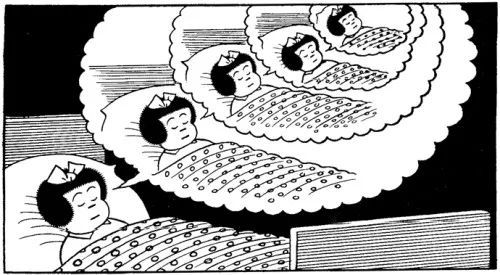
\includegraphics[scale=0.7]{img/Chapter5/5-4/1.png}
\end{figure}

\vspace{0.5cm}

\mybox{讲故事}

\begin{lstlisting}[language=Python]
def tell_story():
    story = "从前有座山,山里有座庙\n"
    story += "庙里有个老和尚\n"
    story += "老和尚在对小和尚讲故事:\n"
    print(story)

    tell_story()

def main():
    tell_story()

if __name__ == "__main__":
    main()
\end{lstlisting}

\begin{tcolorbox}
	\mybox{运行结果}
	\begin{verbatim}
从前有座山,山里有座庙
庙里有个老和尚
老和尚在对小和尚讲故事:
从前有座山,山里有座庙
庙里有个老和尚
老和尚在对小和尚讲故事:
从前有座山,山里有座庙
庙里有个老和尚
老和尚在对小和尚讲故事:
...
	\end{verbatim}
\end{tcolorbox}

一个永远无法结束的递归函数最终会导致栈溢出。因此递归函数需要确定一个结束条件,确保在递归过程中能在合适的地方停止并返回。\\

\mybox{阶乘}

\begin{lstlisting}[language=Python]
def factorial(n):
    if n == 0 or n == 1:
        return 1
    return n * factorial(n-1)

def main():
    print("5! =", factorial(5))

if __name__ == "__main__":
    main()
\end{lstlisting}

\begin{tcolorbox}
	\mybox{运行结果}
	\begin{verbatim}
5! = 120
	\end{verbatim}
\end{tcolorbox}

\begin{figure}[H]
	\centering
	\begin{tikzpicture}[]
		\draw (0,0) rectangle (3,1.5);
		\draw (3,-2) rectangle (6,-0.5);
		\draw (6,-4) rectangle (9,-2.5);
		\draw (9,-6) rectangle (12,-4.5);
		\draw (12,-8) rectangle (15,-6.5);

		\draw (12.75,-10.75) rectangle (14.25,-9.25);
		\draw (9.75,-8.75) rectangle (11.25,-7.25);
		\draw (6.75,-6.75) rectangle (8.25,-5.25);
		\draw (3.75,-4.75) rectangle (5.25,-3.25);
		\draw (0.75,-2.75) rectangle (2.25,-1.25);

		\draw (1.5,0.75) node {$ factorial(5) $};
		\draw (4.5,-1.25) node {$ factorial(4) $};
		\draw (7.5,-3.25) node {$ factorial(3) $};
		\draw (10.5,-5.25) node {$ factorial(2) $};
		\draw (13.5,-7.25) node {$ factorial(1) $};

		\draw (13.5,-10) node {$ 1 $};
		\draw (10.5,-8) node {$ 2 $};
		\draw (7.5,-6) node {$ 6 $};
		\draw (4.5,-4) node {$ 24 $};
		\draw (1.5,-2) node {$ 120 $};

		\draw[->] (3,0.75) -- (4.5,0.75) -- (4.5,-0.5);
		\draw[->] (6,-1.25) -- (7.5,-1.25) -- (7.5,-2.5);
		\draw[->] (9,-3.25) -- (10.5,-3.25) -- (10.5,-4.5);
		\draw[->] (12,-5.25) -- (13.5,-5.25) -- (13.5,-6.5);

		\draw[->] (12.75,-10) -- (10.5,-10) -- (10.5,-8.75);
		\draw[->] (9.75,-8) -- (7.5,-8) -- (7.5,-6.75);
		\draw[->] (6.75,-6) -- (4.5,-6) -- (4.5,-4.75);
		\draw[->] (3.75,-4) -- (1.5,-4) -- (1.5,-2.75);

		\draw (4.5,1) node {$ 5 * factorial(4) $};
		\draw (7.5,-1) node {$ 4 * factorial(3) $};
		\draw (10.5,-3) node {$ 3 * factorial(2) $};
		\draw (13.5,-5) node {$ 2 * factorial(1) $};

		\draw (11,-10.5) node {$ 2 * 1 $};
		\draw (8,-8.5) node {$ 3 * 2 $};
		\draw (5,-6.5) node {$ 4 * 6 $};
		\draw (2,-4.5) node {$ 5 * 24 $};
	\end{tikzpicture}
	\caption{阶乘}
\end{figure}

\vspace{0.5cm}

\mybox{斐波那契数列}

\begin{lstlisting}[language=Python]
def fibonacci(n):
    if n == 1 or n == 2:
        return n
    return fibonacci(n-2) + fibonacci(n-1)

def main():
    n = 7
    print(fibonacci(n))

if __name__ == "__main__":
    main()
\end{lstlisting}

\begin{tcolorbox}
	\mybox{运行结果}
	\begin{verbatim}
21
	\end{verbatim}
\end{tcolorbox}

\begin{figure}[H]
	\centering
	\begin{tikzpicture}[
			level distance=2.4cm,
			level 1/.style={sibling distance=6cm},
			level 2/.style={sibling distance=3cm},
			level 3/.style={sibling distance=2cm}
		]
		\node {$ f(5) $}
		child {
				node {$ f(3) $}
				child {node {$ f(1) $}}
				child {node {$ f(2) $}}
			}
		child {
				node {$ f(4) $}
				child {node {$ f(2) $}}
				child {
						node {$ f(3) $}
						child {node {$ f(1) $}}
						child {node {$ f(2) $}}
					}
			};
	\end{tikzpicture}
	\caption{递归树}
\end{figure}

递归的特点就是将一个复杂的大问题逐步简化为一个可以解决的小问题,然后再逐步计算出大问题的解。\\

递归的优点在于代码简洁易懂,但是缺点也很明显,就是效率很低。每次递归都会产生函数调用,而函数调用的开销是很大的,不适合用来解决大规模的问题。\\

例如在计算斐波那契数列的第40项时,递归需要花费大量时间,因为其中包含了大量的重复计算。相比而言,使用循环的方式能够节省大量的时间。因此像阶乘和斐波那契数列这样的情况,通常会采用循环,而不是递归进行计算。\\

然而还存在很多问题不得不使用递归的思想才能解决。\\

\mybox{阿克曼函数}

\begin{align}\nonumber
	A(m, n) =
	\begin{cases}
		n + 1             & m = 0        \\
		A(m-1, 1)         & m > 0, n = 0 \\
		A(m-1, A(m, n-1)) & m > 0, n > 0 \\
	\end{cases}
\end{align}

\begin{lstlisting}[language=Python]
def A(m, n):
    if m == 0:
        return n + 1
    elif m > 0 and n == 0:
        return A(m - 1, 1)
    else:
        return A(m - 1, A(m, n - 1))

def main():
    print(A(3, 4))

if __name__ == "__main__":
    main()
\end{lstlisting}

\begin{tcolorbox}
	\mybox{运行结果}
	\begin{verbatim}
125
	\end{verbatim}
\end{tcolorbox}

\vspace{0.5cm}

\mybox{汉诺塔}\\

有三根柱子A、B、C,A柱子上从下到上套有n个圆盘,要求将A柱子上的圆盘移动到C柱子上。每次只能移动一个圆盘,且大圆盘始终不能叠在小圆盘上面。\\

\begin{figure}[H]
	\centering
	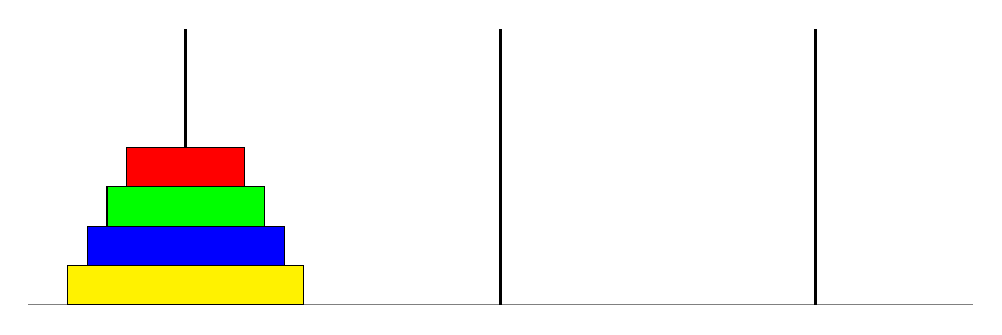
\begin{tikzpicture}[scale=0.5]
		\draw[-, gray] (0,0) -- (24,0);
		\draw[-, very thick] (4,0) -- (4,7);
		\draw[-, very thick] (12,0) -- (12,7);
		\draw[-, very thick] (20,0) -- (20,7);

		\draw[fill=red] (2.5,3) rectangle (5.5,4);
		\draw[fill=green] (2,2) rectangle (6,3);
		\draw[fill=blue] (1.5,1) rectangle (6.5,2);
		\draw[fill=yellow] (1,0) rectangle (7,1);
	\end{tikzpicture}
	\caption{汉诺塔}
\end{figure}

递归算法求解汉诺塔问题:

\begin{enumerate}
	\item 将n-1个圆盘从A借助C移到B。
	\item 将第n个圆盘从A移到C。
	\item 将n-1个圆盘从B借助A移到C。
\end{enumerate}

\vspace{-0.5cm}

\begin{lstlisting}[language=Python]
move = 0

def hanoi(n, src, mid, dst):
	global move

	if n == 1:
		print(src, "->", dst)
		move += 1
	else:
		# move top n-1 disks from src to mid
		hanoi(n - 1, src, dst, mid)
		print(src, "->", dst)
		move += 1
		# move top n-1 disks from mid to dst
		hanoi(n - 1, mid, src, dst)

def main():
	hanoi(3, "A", "B", "C")
	print("Moves:", move)

if __name__ == "__main__":
	main()
\end{lstlisting}

\begin{tcolorbox}
	\mybox{运行结果}
	\begin{verbatim}
A -> C
A -> B
C -> B
A -> C
B -> A
B -> C
A -> C
Moves: 7
	\end{verbatim}
\end{tcolorbox}

假设每次移动花费1秒,解决一个64层的汉诺塔问题大约需要5800亿年。\\

\begin{figure}[H]
	\centering
	
\includegraphics[]{img/Chapter5/5-4/2.png}
\end{figure}

\newpage
\chapter{模块}

\section{random}

\subsection{random}

random模块提供了生成随机数据的功能。

\begin{table}[H]
    \centering
    \setlength{\tabcolsep}{5mm}{
        \begin{tabular}{|l|l|}
            \hline
            \textbf{方法} & \textbf{功能}                      \\
            \hline
            random()      & 生成一个$ [0, 1] $之间的随机浮点数 \\
            \hline
            randint(x, y) & 生成一个$ [x, y] $之间的随机整数   \\
            \hline
            choice()      & 从序列中随机返回一个元素           \\
            \hline
            shuffle()     & 将序列打乱                         \\
            \hline
            sample()      & 从序列中生成一组唯一的随机元素     \\
            \hline
        \end{tabular}
    }
    \caption{random模块}
\end{table}

\mybox{随机密码生成}

\begin{lstlisting}[language=Python]
import random
import string

def password_generator(length):
    characters = string.ascii_letters + string.digits
    return "".join(random.choice(characters) for _ in range(length))

def main():
    length = int(input("Enter length of password: "))
    print(password_generator(length))

if __name__ == "__main__":
    main()
\end{lstlisting}

\begin{tcolorbox}
    \mybox{运行结果}
    \begin{verbatim}
Enter length of password: 8
@o8VBuiV
\end{verbatim}
\end{tcolorbox}

\newpage

\section{copy}

\subsection{copy}

copy是一个专门进行内容复制的处理模块。拷贝分为浅拷贝(shallow copy)和深拷贝(deep copy)两种:

\begin{itemize}
    \item 浅拷贝:只是复制第一层的内容,而更深入的数据嵌套关系不会拷贝。
    \item 深拷贝:会进行完整的复制。
\end{itemize}

\vspace{0.5cm}

\subsection{引用}

引用的本质在于将同一块内存空间,交给不同的对象进行同时操作,当一个对象修改了内存数据之后,其它对象的内存数据也会同时发生改变。

\vspace{-0.5cm}

\begin{lstlisting}[language=Python]
a = {1:[1, 2, 3]}
b = a
\end{lstlisting}

\begin{figure}[H]
    \centering
    \begin{tikzpicture}
        \draw (0,0) rectangle node{\{1:\textcolor{blue}{[1, 2, 3]}\}} (2.5,1);
        \draw (-2,1.5) circle(0.5) node{a};
        \draw (-2,-0.5) circle(0.5) node{b};
        \draw (3,-2) rectangle node{\textcolor{blue}{[1, 2, 3]}} (5,-1);

        \draw[->] (-1.5,1.5) -- (0,1);
        \draw[->] (-1.5,-0.5) -- (0,0);
        \draw[->, blue] (1.4,0.2) -- (1.4,-1.5) -- (3,-1.5);
    \end{tikzpicture}
    \caption{引用}
\end{figure}

\vspace{0.5cm}

\mybox{引用传递}

\begin{lstlisting}[language=Python]
def main():
    info = dict(name="小灰", age=16, skills=["Python", "C/C++"])
    copy_info = info        # 引用传递
    copy_info["skills"].append("Java")
    print(info)

if __name__ == "__main__":
    main()
\end{lstlisting}

\begin{tcolorbox}
    \mybox{运行结果}
    \begin{verbatim}
{'name':'小灰', 'age':16, 'skills':['Python', 'C/C++', 'Java']}
\end{verbatim}
\end{tcolorbox}

\vspace{0.5cm}

\subsection{浅拷贝}

拷贝和引用传递是不同的,拷贝是将原始的内存的数据进行一份复制,而后为其分配单独的对象的指向。

\vspace{-0.5cm}

\begin{lstlisting}[language=Python]
a = {1:[1, 2, 3]}
b = a.copy()
\end{lstlisting}

\begin{figure}[H]
    \centering
    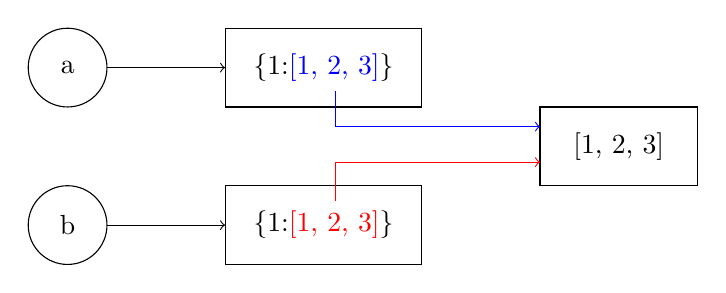
\begin{tikzpicture}
        \draw (0,1) rectangle node{\{1:\textcolor{blue}{[1, 2, 3]}\}} (2.5,2);
        \draw (-2,1.5) circle(0.5) node{a};
        \draw (0,-1) rectangle node{\{1:\textcolor{red}{[1, 2, 3]}\}} (2.5,0);
        \draw (-2,-0.5) circle(0.5) node{b};
        \draw (4,0) rectangle node{[1, 2, 3]} (6,1);

        \draw[->] (-1.5,1.5) -- (0,1.5);
        \draw[->] (-1.5,-0.5) -- (0,-0.5);
        \draw[->, blue] (1.4,1.2) -- (1.4,0.75) -- (4,0.75);
        \draw[->, red] (1.4,-0.2) -- (1.4,0.3) -- (4,0.3);
    \end{tikzpicture}
    \caption{浅拷贝}
\end{figure}

\vspace{0.5cm}

\mybox{浅拷贝}

\begin{lstlisting}[language=Python]
import copy

def main():
    info = dict(name="小灰", age=16, skills=["Python", "C/C++"])
    copy_info = copy.copy(info)     # 浅拷贝
    copy_info.pop("age")
    copy_info["skills"].append("Java")
    print(info)
    print(copy_info)

if __name__ == "__main__":
    main()
\end{lstlisting}

\begin{tcolorbox}
    \mybox{运行结果}
    \begin{verbatim}
{'name':'小灰', 'age':16, 'skills':['Python', 'C/C++', 'Java']}
{'name':'小灰', 'skills':['Python', 'C/C++', 'Java']}
\end{verbatim}
\end{tcolorbox}

\vspace{0.5cm}

\subsection{深拷贝}

\vspace{-0.5cm}

\begin{lstlisting}[language=Python]
a = {1:[1, 2, 3]}
b = copy.deepcopy(a)
\end{lstlisting}

\begin{figure}[H]
    \centering
    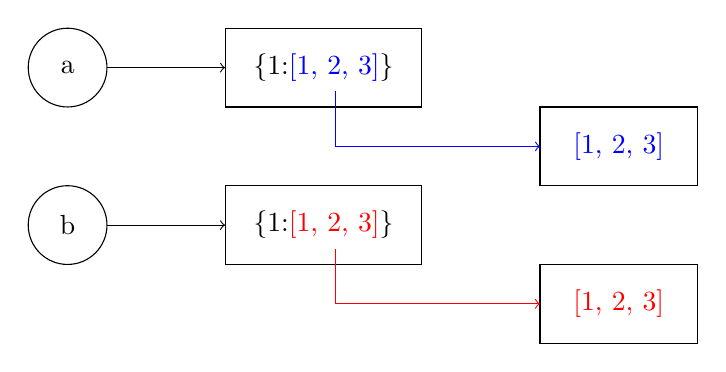
\begin{tikzpicture}
        \draw (0,1) rectangle node{\{1:\textcolor{blue}{[1, 2, 3]}\}} (2.5,2);
        \draw (-2,1.5) circle(0.5) node{a};
        \draw (0,-1) rectangle node{\{1:\textcolor{red}{[1, 2, 3]}\}} (2.5,0);
        \draw (-2,-0.5) circle(0.5) node{b};
        \draw (4,0) rectangle node{\textcolor{blue}{[1, 2, 3]}} (6,1);
        \draw (4,-2) rectangle node{\textcolor{red}{[1, 2, 3]}} (6,-1);

        \draw[->] (-1.5,1.5) -- (0,1.5);
        \draw[->] (-1.5,-0.5) -- (0,-0.5);
        \draw[->, blue] (1.4,1.2) -- (1.4,0.5) -- (4,0.5);
        \draw[->, red] (1.4,-0.8) -- (1.4,-1.5) -- (4,-1.5);
    \end{tikzpicture}
    \caption{深拷贝}
\end{figure}

\vspace{0.5cm}

\mybox{深拷贝}

\begin{lstlisting}[language=Python]
import copy

def main():
    info = dict(name="小灰", age=16, skills=["Python", "C/C++"])
    copy_info = copy.deepcopy(info)     # 深拷贝
    copy_info.pop("age")
    copy_info["skills"].append("Java")
    print(info)
    print(copy_info)

if __name__ == "__main__":
    main()
\end{lstlisting}

\begin{tcolorbox}
    \mybox{运行结果}
    \begin{verbatim}
{'name': '小灰', 'age': 16, 'skills': ['Python', 'C/C++']}
{'name': '小灰', 'skills': ['Python', 'C/C++', 'Java']}
\end{verbatim}
\end{tcolorbox}

\newpage

\section{MapReduce数据处理}

\subsection{MapReduce}

Python在数据分析领域上使用非常广泛,并且实现简单。在Python中可以进行大量数据的快速处理,进行数据的过滤、分析操作。在数据量小的情况下可以方便地使用for循环进行数据的逐个处理,但是在数据量大的情况下,就需要使用一些特定的处理函数进行过滤、分析、统计等操作。\\

在Python中默认提供有了filter()、map(),但是要进行统计处理,则需要导入reduce()。

\begin{table}[H]
    \centering
    \setlength{\tabcolsep}{5mm}{
        \begin{tabular}{|l|l|}
            \hline
            \textbf{函数}              & \textbf{功能}            \\
            \hline
            filter(function, sequence) & 对传入的序列数据进行过滤 \\
            \hline
            map(function, sequence)    & 对传入的序列数据进行处理 \\
            \hline
            reduce(function, sequence) & 对传入的序列数据进行统计 \\
            \hline
        \end{tabular}
    }
    \caption{MapReduce数据处理函数}
\end{table}

在进行数据处理的过程之中都需要有一个处理函数,这个处理函数就定义了数据该如何进行处理或统计,一般而言这样的函数都比较短,所以大部分情况下都可以利用lambda函数来完成。\\

\mybox{MapReduce数据处理}

\begin{lstlisting}[language=Python]
from functools import reduce

def main():
    lst = list(range(10))

    filter_lst = list(filter(lambda x: x % 2 ==0, lst))
    print("过滤出偶数:%s" % filter_lst)

    map_lst = list(map(lambda x: x ** 2, filter_lst))
    print("平方:%s" % map_lst)

    result = reduce(lambda x, y: x+y, map_lst)
    print("求和:%d" % result)

if __name__ == "__main__":
    main()
\end{lstlisting}

\begin{tcolorbox}
    \mybox{运行结果}
    \begin{verbatim}
过滤出偶数:[0, 2, 4, 6, 8]
平方:[0, 4, 16, 36, 64]
求和:120
\end{verbatim}
\end{tcolorbox}

\newpage

\section{jieba}

\subsection{pip}

Python本地有一些系统模块开发者可以直接进行使用,但是开发者仅仅是依靠系统模块是不够的,需要大量的使用第三方模块。为了解决这些模块的管理问题,在Python中内置了pip管理工具。通过此工具可以直接连接到Python远程服务模块仓库,通过仓库下载所需要的模块。\\

在Python安装的时候会自动进行pip工具的相关安装,输入pip --help查看pip的相关命令选项。

\begin{table}[H]
    \centering
    \setlength{\tabcolsep}{5mm}{
        \begin{tabular}{|l|l|}
            \hline
            \textbf{功能}  & \textbf{命令}                \\
            \hline
            搜索模块       & pip search 模块名            \\
            \hline
            安装模块       & pip install 模块名           \\
            \hline
            查看已安装模块 & pip list                     \\
            \hline
            列出过期模块   & pip list --outdated          \\
            \hline
            更新模块       & pip install --upgrade 模块名 \\
            \hline
            卸载模块       & pip uninstall 模块名         \\
            \hline
        \end{tabular}
    }
    \caption{pip命令}
\end{table}

\vspace{0.5cm}

\subsection{jieba}

分词是一种数学的应用,它可以直接根据词语之间的数学关系进行文字或单词的抽象。例如对“中华人民共和国”进行分词处理,可以拆分为“中华”、“华人”、“人民”、“共和”、“共和国”、“中华人民共和国”。如果没有分词,就无法进行搜索引擎的开发。\\

jieba是在中文自然语言处理中用得最多的工具包之一,它以分词起家,目前已经能够实现包括分词、词性标注以及命名实体识别等多种功能。\\

考虑到分词的效果与性能,在jieba组件中提供有3种分词模式:

\begin{enumerate}
    \item 精确模式:将句子进行最精确的切分,分词速度相对较低。

    \item 全模式:基于词汇列表将句子中所有可以成词的词语都扫描出来,该模式处理速度非常快,但是不能有效解决歧义的问题。

    \item 搜索引擎模式:在精确模式的基础上,对长词进行再次切分,该模式适用于搜索引擎构建索引的分词。
\end{enumerate}

\vspace{0.5cm}

\mybox{统计《西游记》中出现次数最多的20个词语}

\begin{lstlisting}[language=Python]
import jieba

PATH = "西游记.txt"     # 文件路径

def main():
    word_frequence = {}     # 词频表

    # 打开文件
    with open(file=PATH, mode="r", encoding="UTF-8") as file:
        line = file.readline()  # 读取一行数据
        while line:
            words = jieba.lcut(line)    # 分词
            for word in words:
                if len(word) == 1:  # 舍弃长度为1的词
                    continue
                else:
                    # dict.get(key, default=None)
                    word_frequence[word] 
                        = word_frequence.get(word, 0) + 1
            line = file.readline()

        # 获取所有数据项
        items = list(word_frequence.items())
        # 根据出现次数降序排序
        items.sort(key=lambda x: x[1], reverse=True)

        # 取前20项
        for i in range(20):
            word, count = items[i]
            print("%s: %s" % (word, count))

if __name__ == "__main__":
    main()
\end{lstlisting}

\newpage
\chapter{面向过程}

\section{面向过程与面向对象}

\subsection{面向过程(Procedure Oriented)}

面向过程是一种以过程为中心的编程思想,以什么正在发生为主要目标进行编程,分析出解决问题所需要的步骤,然后用函数把这些步骤一步一步实现,使用的时候一个一个依次调用。\\

C语言就是一种面向过程的编程语言,但是面向过程的缺陷是数据和函数并不完全独立,使用两个不同的实体表示信息及其操作。\\

\subsection{面向对象(Object Oriented)}

面向对象是相对于面向过程来讲的,面向对象方法把相关的数据和方法组织为一个整体来看待,从更高的层次来进行系统建模,更贴近事物的自然运行模式。\\

在面向对象中,把构成问题的事物分解成各个对象,建立对象的目的不是为了完成一个步骤,而是为了描叙某个事物在整个解决问题的步骤中的行为。\\

Java、C++、Python等都是面向对象的编程语言,面向对象的优势在于只是用一个实体就能同时表示信息及其操作。\\

面向对象三大特性:

\begin{enumerate}
	\item 封装(encapsulation):数据和代码捆绑,避免外界干扰和不确定性访问。
	\item 继承(inheritance):让某种类型对象获得另一类型对象的属性和方法。
	\item 多态(polymorphism):同一事物表现出不同事物的能力。
\end{enumerate}

\newpage

\section{类与对象}

\subsection{类与对象}

类(class)表示同一类具有相同特征和行为的对象的集合,类定义了对象的属性和方法。\\

对象(object)是类的实例,对象拥有属性和方法。\\

类的设计需要使用关键字class,类名是一个标识符,遵循大驼峰命名法。类中可以包含属性和方法。其中,属性通过变量表示,又称实例变量;方法用于描述行为,又称实例方法。\\

在程序之中如果需要使用类,那么一般都会通过对象来进行操作。

\vspace{-0.5cm}

\begin{lstlisting}[language=Python]
obj_name = class_name([param])
\end{lstlisting}

当实例化了一个对象之后,就可以通过此对象进行类中成员的访问:

\begin{itemize}
	\item 对象.属性:访问类中的属性内容,如果程序中访问了没有定义的实例属性,那么将引发AttributeError异常。

	\item 对象.方法():调用类中的方法。对于类中每一个方法的当前对象都会有Python自己来负责该对象的传入,这一操作不是由用户负责的。
\end{itemize}

\vspace{0.5cm}

\mybox{类和对象}

\begin{lstlisting}[language=Python]
class Person:
    name = ""
    age = 0
    gender = ""

    def eat(self):
        print("吃饭")
    
    def sleep(self):
        print("睡觉")

def main():
    person = Person()
    
    person.name = "小灰"
    person.age = 16
    person.gender = "男"
    
    print("姓名:%s,年龄:%d,性别:%s" % (
            person.name, person.age, person.gender))
    person.eat()
    person.sleep()

if __name__ == "__main__":
    main()
\end{lstlisting}

\begin{tcolorbox}
	\mybox{运行结果}
	\begin{verbatim}
姓名:小灰,年龄:16,性别:男
吃饭
睡觉
\end{verbatim}
\end{tcolorbox}

\vspace{0.5cm}

\subsection{垃圾回收机制}

引用传递的本质在于将同一块空间修改权力交由不同的对象来完成,在这样的处理之中就有可能产生垃圾空间。在Python的引用数据处理之中都会存在有一个引用计数器,当引用计数器为0的时候就表示该对象已经成为了垃圾,等待进行回收。\\

\mybox{垃圾回收机制}

\begin{lstlisting}[language=Python]
class Person:
    pass

def main():
    person1 = Person()
    person2 = Person()

    print("【引用传递前地址】person1: %d, person2: %d" % (
            id(person1), id(person2)))
    person2 = person1
    print("【引用传递后地址】person1: %d, person2: %d" % (
            id(person1), id(person2)))

if __name__ == "__main__":
    main()
\end{lstlisting}

\begin{tcolorbox}
	\mybox{运行结果}
	\begin{verbatim}
【引用传递前地址】person1: 1988221852552, person2: 1988222686536
【引用传递后地址】person1: 1988221852552, person2: 1988221852552
\end{verbatim}
\end{tcolorbox}

在开发之中,实际上对于垃圾空间应该尽可能少的产生,虽然Python提供有垃圾收集机制,但是垃圾的回收与释放依然需要占用系统资源。

\newpage

\section{封装}

\subsection{封装(Encapsulation)}

封装是面向对象方法的重要原则,就是把对象的属性和方法结合为一个独立的整体,并尽可能隐藏对象的内部实现细节。\\

封装可以认为是一个保护屏障,防止该类的数据被外部类随意访问。要访问该类的数据,必须通过严格的接口控制。合适的封装可以让代码更容易理解和维护,也加强了程序的安全性。\\

实现封装的步骤:

\begin{enumerate}
	\item 修改属性的可见性来限制对属性的访问,一般限制为private。
	\item 对每个属性提供对外的公共方法访问,也就是提供一对setter / getter,用于对私有属性的访问。
\end{enumerate}

\vspace{0.5cm}

\mybox{封装}

\begin{lstlisting}[language=Python]
class Person:
    def set_name(self, name):
        self.__name = name
    
    def get_name(self):
        return self.__name
    
    def set_age(self, age):
        self.__age = age
    
    def get_age(self):
        return self.__age

def main():
    person = Person()
    person.set_name("小灰")
    person.set_age(17)
    print("姓名:%s,年龄:%d" % (
            person.get_name(), person.get_age()))

if __name__ == "__main__":
    main()
\end{lstlisting}

\begin{tcolorbox}
	\mybox{运行结果}
	\begin{verbatim}
姓名:小灰,年龄:17
\end{verbatim}
\end{tcolorbox}

\newpage

\section{构造方法与析构方法}

\subsection{构造方法(Constructor)}

构造方法也是一个方法,用于实例化对象,在实例化对象的时候调用。一般情况下,使用构造方法是为了在实例化对象的同时,给一些属性进行初始化赋值。\\

构造方法和普通方法的区别:

\begin{enumerate}
	\item 构造方法的名称必须为\_\_init\_\_()。
	\item 构造方法没有返回值。
	\item 一个类中只允许定义最多1个构造方法。
\end{enumerate}

如果一个类中没有写构造方法,系统会自动提供一个无参构造方法,以便实例化对象。\\

\mybox{构造方法}

\begin{lstlisting}[language=Python]
class Person:
    def __init__(self, name, age):
        self.__name = name
        self.__age = age
    
    def get_info(self):
        return "姓名:%s,年龄:%d" % (self.__name, self.__age)

def main():
    person = Person("小灰", 17)
    print(person.get_info())

if __name__ == "__main__":
    main()
\end{lstlisting}

\begin{tcolorbox}
	\mybox{运行结果}
	\begin{verbatim}
姓名:小灰,年龄:17
\end{verbatim}
\end{tcolorbox}

\vspace{0.5cm}

\subsection{析构方法(Destructor)}

在对象实例化的时候会触发构造方法的执行,与之对应的操作称为析构,当对象不再使用的时候进行某些收尾处理的操作。析构方法名称也要要求,必须为\_\_del\_\_()。\\

\mybox{析构方法}

\begin{lstlisting}[language=Python]
class Person:
    def __init__(self):
        print("构造方法被执行了")
    
    def __del__(self):
        print("析构方法被执行了")

def main():
    person = Person()
    del person

if __name__ == "__main__":
    main()
\end{lstlisting}

\begin{tcolorbox}
	\mybox{运行结果}
	\begin{verbatim}
构造方法被执行了
析构方法被执行了
\end{verbatim}
\end{tcolorbox}

\vspace{0.5cm}

\subsection{匿名对象}

对象的名称只是一个地址的信息,真正的内容是保存在内存中的,如果不需要名称就可以使用匿名对象。匿名对象使用完成之后由于没有其它对象进行引用,那么就有可能被垃圾回收,同时也会调用析构方法。\\

如果一个对象要被反复使用,那么可以定义有名对象;如果一个对象只是用一次,就采用匿名对象完成操作即可。\\

\mybox{匿名对象}

\begin{lstlisting}[language=Python]
class Person:
    def __init__(self, name, age):
        self.__name = name
        self.__age = age
    
    def get_info(self):
        return "姓名:%s,年龄:%d" % (self.__name, self.__age)

def main():
    print(Person("小灰", 17).get_info())

if __name__ == "__main__":
    main()
\end{lstlisting}

\begin{tcolorbox}
	\mybox{运行结果}
	\begin{verbatim}
姓名:小灰,年龄:17
\end{verbatim}
\end{tcolorbox}

\newpage

\section{继承}

\subsection{继承(Inheritance)}

继承是面向对象的三大特征之一,程序中的继承是类与类之间的特征和行为的一种赠予或获取。两个类之间的继承必须满足“is a”的关系。子类继承自父类,父类也称基类或超类,子类也称派生类。

\begin{figure}[H]
	\centering
	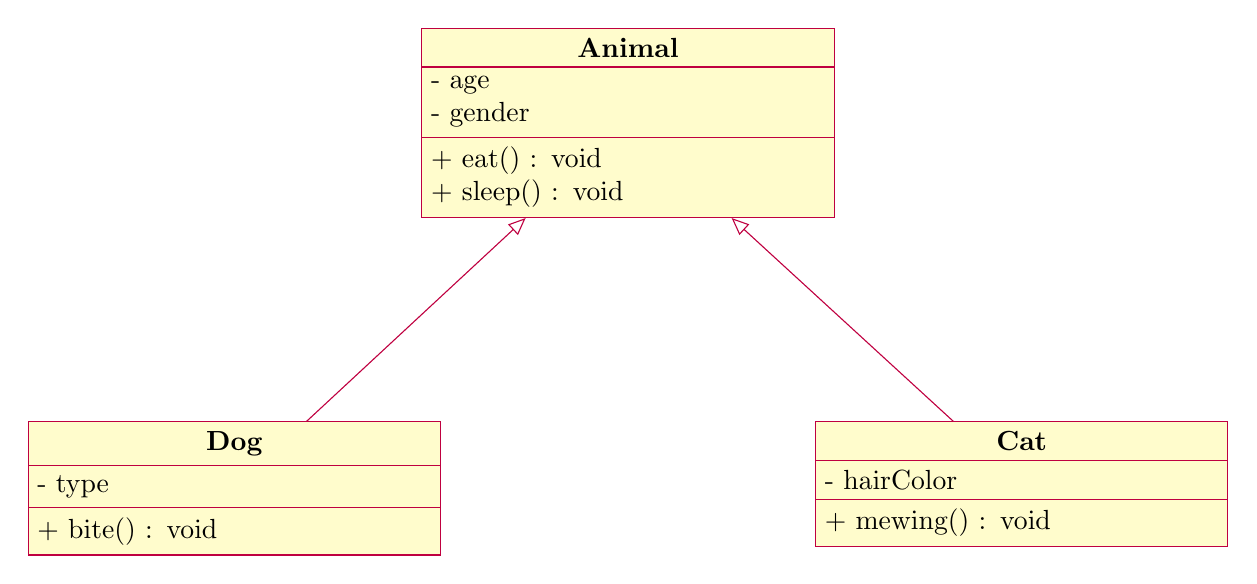
\begin{tikzpicture}
		\begin{class}{Animal}{0,0}
			\attribute{- age}
			\attribute{- gender}
			\operation{+ eat() : void}
			\operation{+ sleep() : void}
		\end{class}

		\begin{class}{Dog}{-5,-5}
			\inherit{Animal}
			\attribute{- type}
			\operation{+ bite() : void}
		\end{class}

		\begin{class}{Cat}{5,-5}
			\inherit{Animal}
			\attribute{- hairColor}
			\operation{+ mewing() : void}
		\end{class}
	\end{tikzpicture}
	\caption{继承}
\end{figure}

产生继承关系后,子类可以使用父类中的属性和方法,也可以定义子类独有的属性和方法。

\vspace{-0.5cm}

\begin{lstlisting}[language=Python]
class subclass(superclass1, ...):
    # code
\end{lstlisting}

在进行继承的时候,子类会继承父类之中全部定义的结构。但是对于构造方法的继承是比较特殊的,需要考虑两种情况:

\begin{enumerate}
	\item 当父类定义了构造方法,但是子类没有定义构造方法时,实例化子类对象会自动调用父类中提供的无参构造方法。

	\item 当子类定义了构造方法时,将不再默认调用父类中的任何构造方法,但是可以手动调用。如果有需要也可以通过super类的实例实现子类调用父类结构的需求。
\end{enumerate}

\vspace{0.5cm}

\mybox{继承}

\begin{lstlisting}[language=Python]
class Animal:
    def __init__(self, name, age):
        self.__name = name
        self.__age = age
    
    def set_name(self, name):
        self.__name = name

    def get_name(self):
        return self.__name
    
    def set_age(self, age):
        self.__age = age

    def get_age(self):
        return self.__age

    def eat(self):
        print("吃饭")
    
    def sleep(self):
        print("睡觉")
    
class Dog(Animal):
    def __init__(self, name, age, type):
        super().__init__(name, age)
        self.__type = type
    
    def set_type(self, type):
        self.__type = type

    def get_type(self):
        return self.__type
    
    def bite(self):
        print("咬人")

def main():
    dog = Dog("狗子", 3, "哈士奇")
    
    print("姓名:%s,年龄:%d,品种:%s" % (
            dog.get_name(), dog.get_age(), dog.get_type()))

    dog.eat()
    dog.sleep()
    dog.bite()

if __name__ == "__main__":
    main()
\end{lstlisting}

\begin{tcolorbox}
	\mybox{运行结果}
	\begin{verbatim}
姓名:狗子,年龄:3,品种:哈士奇
吃饭
睡觉
咬人
\end{verbatim}
\end{tcolorbox}

\vspace{0.5cm}

\subsection{多继承}

多继承指一个子类可以同时继承多个父类的内容,在多继承实现中只需要编写多个父类的名称即可。\\

利用多继承的最大优势在于可以在进行子类操作的时候将多个父类中定义的结构全部保留继续使用。\\

\mybox{多继承}

\begin{lstlisting}[language=Python]
class Date:
    def set_date(self, year=1970, month=1, day=1):
        self.__year = year
        self.__month = month
        self.__day = day
    
    def get_date(self):
        return "%04d/%02d/%02d" % (
            self.__year, self.__month, self.__day)
    
class Time:
    def set_time(self, hour=0, minute=0, second=0):
        self.__hour = hour
        self.__minute = minute
        self.__second = second
    
    def get_time(self):
        return "%02d:%02d:%02d" % (
            self.__hour, self.__minute, self.__second)

class DateTime(Date, Time):
    def __init__(self, year=1970, month=1, day=1, 
                       hour=0, minute=0, second=0):
        super().set_date(year, month, day)
        super().set_time(hour, minute, second)
    
    def __repr__(self):
        return super().get_date() + " " + super().get_time()

def main():
    date_time = DateTime(2021, 4, 6, 14, 38, 40)
    print(date_time)

if __name__ == "__main__":
    main()
\end{lstlisting}

\begin{tcolorbox}
	\mybox{运行结果}
	\begin{verbatim}
2021/04/06 14:38:40
\end{verbatim}
\end{tcolorbox}

\newpage

\section{多态}

\subsection{多态(Polymorphism)}

多态是同一个行为具有多个不同表现形式或形态的能力。

\begin{figure}[H]
	\centering
	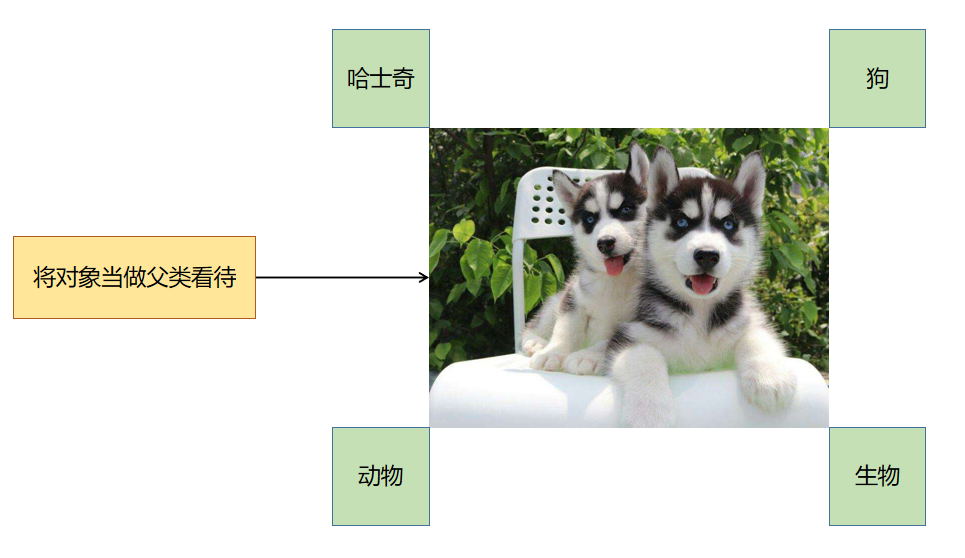
\includegraphics[scale=0.7]{img/C7/7-6/1.png}
	\caption{多态}
\end{figure}

在类继承的结构之中,很难保证父类中的某些操作方法可以被子类继续拿来使用。这个时候子类为保留住原始的方法名称,同时也为了可以对功能实现进一步的扩充,就可以利用方法覆写。\\

\mybox{多态}

\begin{lstlisting}[language=Python]
import math

class Shape:
    def get_area(self):
        pass

class Rectangle(Shape):
    def __init__(self, width, length):
        self.__width = width
        self.__length = length
    
    def get_area(self):
        return self.__length * self.__width

class Circle(Shape):
    def __init__(self, radius):
        self.__radius = radius
    
    def get_area(self):
        return math.pi * self.__radius ** 2

def shape_area(obj):
    if isinstance(obj, Shape):
        return obj.get_area()

def main():
    print("长方形面积:%.2f" % shape_area(Rectangle(6, 11)))
    print("圆形面积:%.2f" % shape_area(Circle(5)))

if __name__ == "__main__":
    main()
\end{lstlisting}

\begin{tcolorbox}
	\mybox{运行结果}
	\begin{verbatim}
长方形面积:66.00
圆形面积:78.54
\end{verbatim}
\end{tcolorbox}

\newpage
\chapter{面向对象}

\section{封装}

\subsection{类与对象}

在面向对象编程中,把构成问题的事物分解成各个对象,每个对象都有自己的数据和行为,程序通过对象之间的交互来实现功能。\\

类(class)是一个模板,定义了对象的属性和方法,用来描述同一类对象的共同特征和行为。对象(object)是类的实例,它具有类定义的属性和方法。\\

实例化一个类对象之后就可以通过访问对象的属性和方法来操作对象。\\

\mybox{银行账户}

\begin{lstlisting}[language=Python]
class BankAccount:
    def deposit(self, amount):
        self.balance += amount
    
    def withdraw(self, amount):
        self.balance -= amount

def main():
    account = BankAccount()
    account.owner = "Terry"
    account.account = "6250941006528599"
    account.balance = 50

    print("Owner:", account.owner)
    print("Account:", account.account)
    print("Balance:", account.balance)

    account.deposit(100)
    print("Balance:", account.balance)

    account.withdraw(70)
    print("Balance:", account.balance)

if __name__ == "__main__":
    main()
\end{lstlisting}

\begin{tcolorbox}
    \mybox{运行结果}
    \begin{verbatim}
Owner: Terry
Account: 6250941006528599
Balance: 50
Balance: 150
Balance: 80
\end{verbatim}
\end{tcolorbox}

\vspace{0.5cm}

\subsection{封装(Encapsulation)}

封装是面向对象的重要原则,尽可能隐藏对象的内部实现细节。封装可以认为是一个保护屏障,防止该类的数据被外部随意访问。当要访问该类的数据时,必须通过指定的接口。合适的封装可以让代码更容易理解和维护,也加强了程序的安全性。\\

为了实现封装,需要对类的属性和方法进行访问权限的控制。通常会将类的属性设置为私有属性,然后对外提供一对setter/getter方法来访问该属性。\\

为了避免方法的参数与类的属性重名造成歧义,可以使用self关键字用来指代当前对象。\\

\mybox{银行账户}

\begin{lstlisting}[language=Python]
class BankAccount:
    __ACCOUNT_DIGITS = 16
    __owner = ""
    __account = ""
    __balance = 0

    def set_owner(self, owner):
        if owner != "":
            self.__owner = owner
    
    def get_owner(self):
        return self.__owner
    
    def set_account(self, account):
        if len(account) == self.__ACCOUNT_DIGITS:
            self.__account = account
    
    def get_account(self):
        return self.__account

    def set_balance(self, balance):
        if balance >= 0:
            self.__balance = balance
    
    def get_balance(self):
        return self.__balance

    def deposit(self, amount):
        if amount <= 0:
            return False
        self.__balance += amount
        return True

    def withdraw(self, amount):
        if amount <= 0 or amount > self.__balance:
            return False
        self.__balance -= amount
        return True

def main():
    account = BankAccount()
    account.set_owner("Terry")
    account.set_account("6250941006528599")
    account.set_balance(50)

    print("Owner:", account.get_owner())
    print("Account:", account.get_account())
    print("Balance:", account.get_balance())

    account.deposit(100)
    print("Balance:", account.get_balance())

    account.withdraw(70)
    print("Balance:", account.get_balance())

if __name__ == "__main__":
    main()
\end{lstlisting}

\begin{tcolorbox}
    \mybox{运行结果}
    \begin{verbatim}
Owner: Terry
Account: 6250941006528599
Balance: 50
Balance: 150
Balance: 80
\end{verbatim}
\end{tcolorbox}

\vspace{0.5cm}

\subsection{构造方法(Constructor)}

构造方法是一种特殊的方法,会在创建对象时自动调用,用于创建并初始化对象,构造方法的名字为\_\_init\_\_()。\\

\mybox{银行账户}

\begin{lstlisting}[language=Python]
class BankAccount:
    def __init__(self, owner, account, balance):
        self.__ACCOUNT_DIGITS = 16
        
        if owner != "":
            self.__owner = owner
        
        if len(account) == self.__ACCOUNT_DIGITS:
            self.__account = account
        
        if balance >= 0:
            self.__balance = balance
    
    def set_owner(self, owner):
        if owner != "":
            self.__owner = owner
    
    def get_owner(self):
        return self.__owner

    def set_account(self, account):
        if len(account) == self.__ACCOUNT_DIGITS:
            self.__account = account

    def get_account(self):
        return self.__account

    def set_balance(self, balance):
        if balance >= 0:
            self.__balance = balance

    def get_balance(self):
        return self.__balance

    def deposit(self, amount):
        if amount <= 0:
            return False
        
        self.__balance += amount
        return True

    def withdraw(self, amount, fee=0):
        if amount <= 0 or amount + fee > self.__balance:
            return False
        
        self.__balance -= amount + fee
        return True

def main():
    account = BankAccount("Terry", "6250941006528599", 50)

    print("Account Balance:", account.get_balance())

    account.withdraw(20)
    print("Account Balance:", account.get_balance())

    account.withdraw(10, 1)
    print("Account Balance:", account.get_balance())

if __name__ == "__main__":
    main()
\end{lstlisting}

\begin{tcolorbox}
    \mybox{运行结果}
    \begin{verbatim}
Account Balance: 50
Account Balance: 30
Account Balance: 19
\end{verbatim}
\end{tcolorbox}

\newpage

\section{继承}

\subsection{继承(Inheritance)}

继承指一个类可以继承另一个类的特征和行为,并可以对其进行扩展。这样就可以避免在多个类中重复定义相同的特征和行为。\\

\begin{figure}[H]
    \centering
    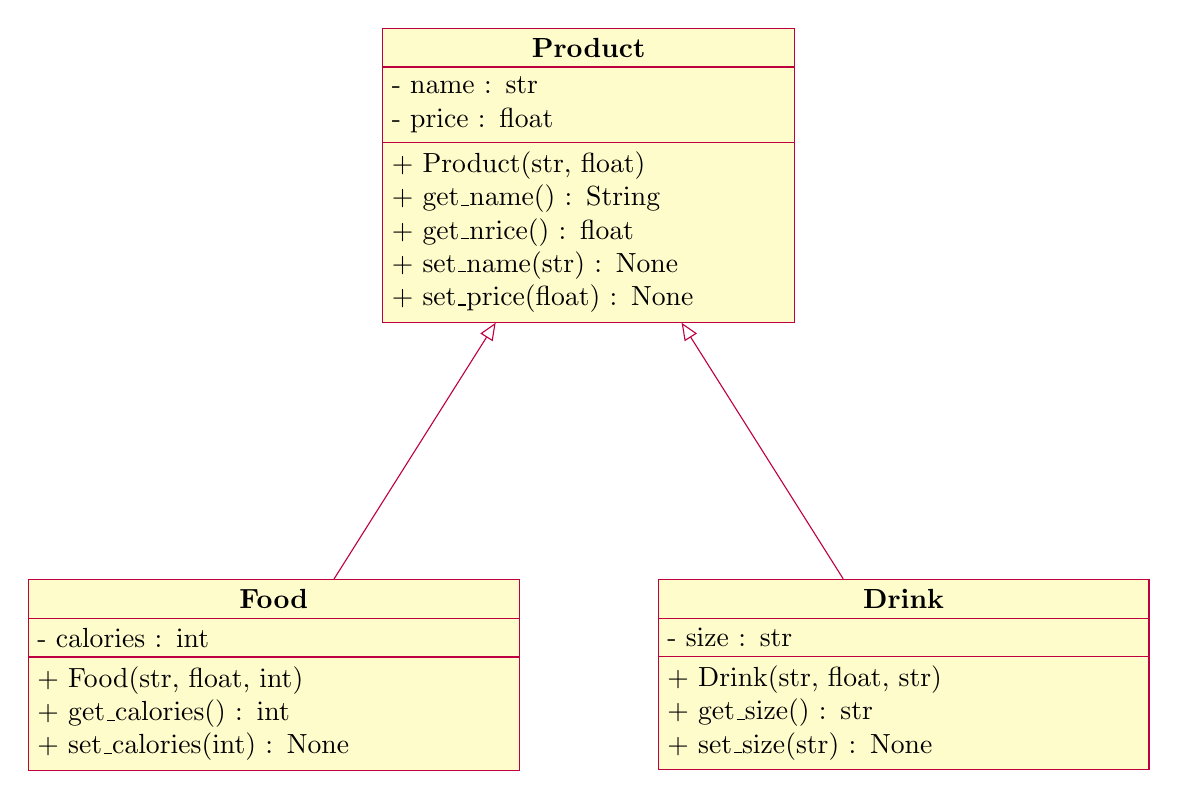
\begin{tikzpicture}
        \begin{class}[text width = 5cm]{Product}{0,0}
            \attribute{- name : str}
            \attribute{- price : float}
            \operation{+ Product(str, float)}
            \operation{+ get\_name() : String}
            \operation{+ get\_nrice() : float}
            \operation{+ set\_name(str) : None}
            \operation{+ set\_price(float) : None}
        \end{class}

        \begin{class}[text width = 6cm]{Food}{-4,-7}
            \inherit{Product}
            \attribute{- calories : int}
            \operation{+ Food(str, float, int)}
            \operation{+ get\_calories() : int}
            \operation{+ set\_calories(int) : None}
        \end{class}

        \begin{class}[text width = 6cm]{Drink}{4,-7}
            \inherit{Product}
            \attribute{- size : str}
            \operation{+ Drink(str, float, str)}
            \operation{+ get\_size() : str}
            \operation{+ set\_size(str) : None}
        \end{class}
    \end{tikzpicture}
    \caption{继承}
\end{figure}

产生继承关系后,子类可以通过super关键字调用父类中的属性和方法,也可以定义子类独有的属性和方法。\\

在创建子类对象时,会先调用父类的构造方法,然后再调用子类的构造方法。因此父类中必须存在一个构造方法,否则将无法创建子类对象。\\

\mybox{麦当劳}

\begin{lstlisting}[language=Python]
class Product:
    def __init__(self, name, price):
        self.__name = name
        self.__price = price
    
    def get_name(self):
        return self.__name
    
    def set_name(self, name):
        self.__name = name

    def get_price(self):
        return self.__price

    def set_price(self, price):
        self.__price = price
\end{lstlisting}

\begin{lstlisting}[language=Python]
from product import Product

class Food(Product):
    def __init__(self, name, price, calories):
        super().__init__(name, price)
        self.__calories = calories
    
    def get_calories(self):
        return self.__calories
    
    def set_calories(self, calories):
        self.__calories = calories
\end{lstlisting}

\begin{lstlisting}[language=Java]
from product import Product

class Drink(Product):
    def __init__(self, name, price, size):
        super().__init__(name, price)
        self.__size = size

    def get_size(self):
        return self.__size

    def set_size(self, size):
        self.__size = size
\end{lstlisting}

\begin{lstlisting}[language=Java]
from food import Food
from drink import Drink

def main():
    food = Food("Cheeseburger", 5.45, 302)
    drink = Drink("Coke", 3.7, "Large")

    print("Food: %s ($%.2f) %d Kcal" % (
        food.get_name(), food.get_price(), food.get_calories())
    )
    print("Drink: %s ($%.2f) %s" % (
        drink.get_name(), drink.get_price(), drink.get_size())
    )

if __name__ == "__main__":
    main()
\end{lstlisting}

\begin{tcolorbox}
    \mybox{运行结果}
    \begin{verbatim}
Food: Cheeseburger ($5.45) 302 Kcal
Drink: Coke ($3.70) Large
	\end{verbatim}
\end{tcolorbox}

\vspace{0.5cm}

\subsection{重写(Override)}

object类是所有类的根类,所有的类都直接或者间接地继承自object类。object类中包含的方法在其它所有类中都可以使用,例如\_\_str\_\_()方法等。\\

当直接输出一个对象时,会自动调用该对象的\_\_str\_\_()方法,将其以字符串的形式输出。

\vspace{-0.5cm}

\begin{lstlisting}[language=Java]
print(food);   # <food.Food object at 0x0000011CE7BC3E10>
\end{lstlisting}

在没有重写\_\_str\_\_()方法的情况下,输出的内容是对象的类名及其地址,但这并不是预期想要的结果。因此,可以重写从父类继承的\_\_str\_\_(),以满足程序的需求。\\

\mybox{麦当劳}

\begin{lstlisting}[language=Python]
class Product:
    def __init__(self, name, price):
        self.__name = name
        self.__price = price
    
    def get_name(self):
        return self.__name
    
    def set_name(self, name):
        self.__name = name

    def get_price(self):
        return self.__price

    def set_price(self, price):
        self.__price = price
    
    def __str__(self):
        return "%s ($%.2f)" % (self.__name, self.__price)
\end{lstlisting}

\begin{lstlisting}[language=Python]
from product import Product

class Food(Product):
    def __init__(self, name, price, calories):
        super().__init__(name, price)
        self.__calories = calories
    
    def get_calories(self):
        return self.__calories
    
    def set_calories(self, calories):
        self.__calories = calories
    
    def __str__(self):
        return "Food: %s %d Kcal" % (
            super().__str__(), self.__calories
        )
\end{lstlisting}

\begin{lstlisting}[language=Python]
from product import Product

class Drink(Product):
    def __init__(self, name, price, size):
        super().__init__(name, price)
        self.__size = size

    def get_size(self):
        return self.__size

    def set_size(self, size):
        self.__size = size
    
    def __str__(self):
        return "Drink: %s %s" % (super().__str__(), self.__size)
\end{lstlisting}

\begin{lstlisting}[language=Python]
from food import Food
from drink import Drink

def main():
    food = Food("Cheeseburger", 5.45, 302)
    drink = Drink("Coke", 3.7, "Large")

    print(food)
    print(drink)

if __name__ == "__main__":
    main()
\end{lstlisting}

\begin{tcolorbox}
    \mybox{运行结果}
    \begin{verbatim}
Food: Cheeseburger ($5.45) 302 Kcal
Drink: Coke ($3.70) Large
	\end{verbatim}
\end{tcolorbox}

\newpage

\section{多态}

\subsection{多态(Polymorphism)}

多态是指对象可以具有多种形态,即同一个对象在不同时刻表现出不同的行为。例如Dog和Cat都是Animal的子类,因此可以将子类对象赋值给父类引用,从而产生多种形态。\\

由子类类型转型为父类类型,称为向上转型。由父类类型转型为子类类型,称为向下转型。\\

\mybox{员工工资}

\begin{lstlisting}[language=Python]
class Employee:
    def __init__(self, name):
        self.__name = name
    
    def get_name(self):
        return self.__name
    
    def set_name(self, name):
        self.__name = name
    
    def get_salary(self):
        pass

class FullTimeEmployee(Employee):
    def __init__(self, name, basic_salary, bonus):
        super().__init__(name)
        self.__basic_salary = basic_salary
        self.__bonus = bonus
    
    def get_salary(self):
        return self.__basic_salary + self.__bonus
    
class PartTimeEmployee(Employee):
    def __init__(self, name, daily_wage, working_days):
        super().__init__(name)
        self.__daily_wage = daily_wage
        self.__working_days = working_days

    def get_salary(self):
        return self.__daily_wage * self.__working_days
\end{lstlisting}

\begin{lstlisting}[language=Python]
from employee import FullTimeEmployee
from employee import PartTimeEmployee

def main():
    employees = [
        FullTimeEmployee('Alice', 5783, 173),
        PartTimeEmployee('Bob', 150, 15)
    ]

    for employee in employees:
        print(
            employee.get_name() + ': $' + str(employee.get_salary())
        )

if __name__ == '__main__':
    main()
\end{lstlisting}

\begin{tcolorbox}
    \mybox{运行结果}
    \begin{verbatim}
Alice: $5956
Bob: $2250
	\end{verbatim}
\end{tcolorbox}

\newpage

\end{document}